%% LyX 2.3.6 created this file.  For more info, see http://www.lyx.org/.
%% Do not edit unless you really know what you are doing.
\documentclass[english,aspectratio=169]{beamer}
\usepackage{lmodern}
\renewcommand{\sfdefault}{lmss}
\renewcommand{\ttdefault}{lmtt}
\usepackage[T1]{fontenc}
\usepackage[latin9]{inputenc}
\setlength{\parskip}{\medskipamount}
\setlength{\parindent}{0pt}
\usepackage{url}
\usepackage{amstext}
\usepackage{amssymb}
\usepackage{graphicx}
\PassOptionsToPackage{normalem}{ulem}
\usepackage{ulem}

\makeatletter

%%%%%%%%%%%%%%%%%%%%%%%%%%%%%% LyX specific LaTeX commands.
\pdfpageheight\paperheight
\pdfpagewidth\paperwidth


%%%%%%%%%%%%%%%%%%%%%%%%%%%%%% Textclass specific LaTeX commands.
% this default might be overridden by plain title style
\newcommand\makebeamertitle{\frame{\maketitle}}%
% (ERT) argument for the TOC
\AtBeginDocument{%
  \let\origtableofcontents=\tableofcontents
  \def\tableofcontents{\@ifnextchar[{\origtableofcontents}{\gobbletableofcontents}}
  \def\gobbletableofcontents#1{\origtableofcontents}
}

%%%%%%%%%%%%%%%%%%%%%%%%%%%%%% User specified LaTeX commands.
\usetheme{CambridgeUS}
\usecolortheme{wolverine}
\hypersetup{}
\usepackage{tikz}
\usepackage{color}
\usepackage{listings}


\makeatother

\usepackage{babel}
\begin{document}
\title[M2]{Vertical properties of geophysical fluids}
\author{Department of Oceanography}
\institute[UCT]{University of Cape Town}
\date{SEA3004F}
\makebeamertitle

\section*{Outline}
\begin{frame}{Outline}

\tableofcontents{}
\end{frame}


\section{The hydrostatic balance}
\begin{frame}{Vertical motion in geophysical fluids}

\begin{columns}[t]


\column{8cm}
\begin{itemize}
\item {\footnotesize{}Fluid motion is driven by pressure differences, which
engender forces (i.e. acceleration) }{\footnotesize\par}
\item {\footnotesize{}Pressure is a mechanical force. Most of the energy
found in the whirls and eddies of the ocean and the atmosphere has
a thermal origin and not just mechanical}{\footnotesize\par}
\item {\footnotesize{}An atmosphere where pressure is the only driver would
be a motionless and stable system. The pressure depends on the weight
of the air column, which is the same everywhere. We say that }\textbf{\footnotesize{}the
lines of equal pressure are also lines of equal gravity force}{\footnotesize{},
known as the geopotential}{\footnotesize\par}
\item {\footnotesize{}In an atmosphere where $\rho=\rho(p,T,\ldots)$ there
can be heating of bottom layers from the Sun that generates movement.
This movement is called }\textbf{\footnotesize{}convection}{\footnotesize{},
in which thermal energy is converted to kinetic energy}{\footnotesize\par}
\end{itemize}

\column{5cm}

{\footnotesize{}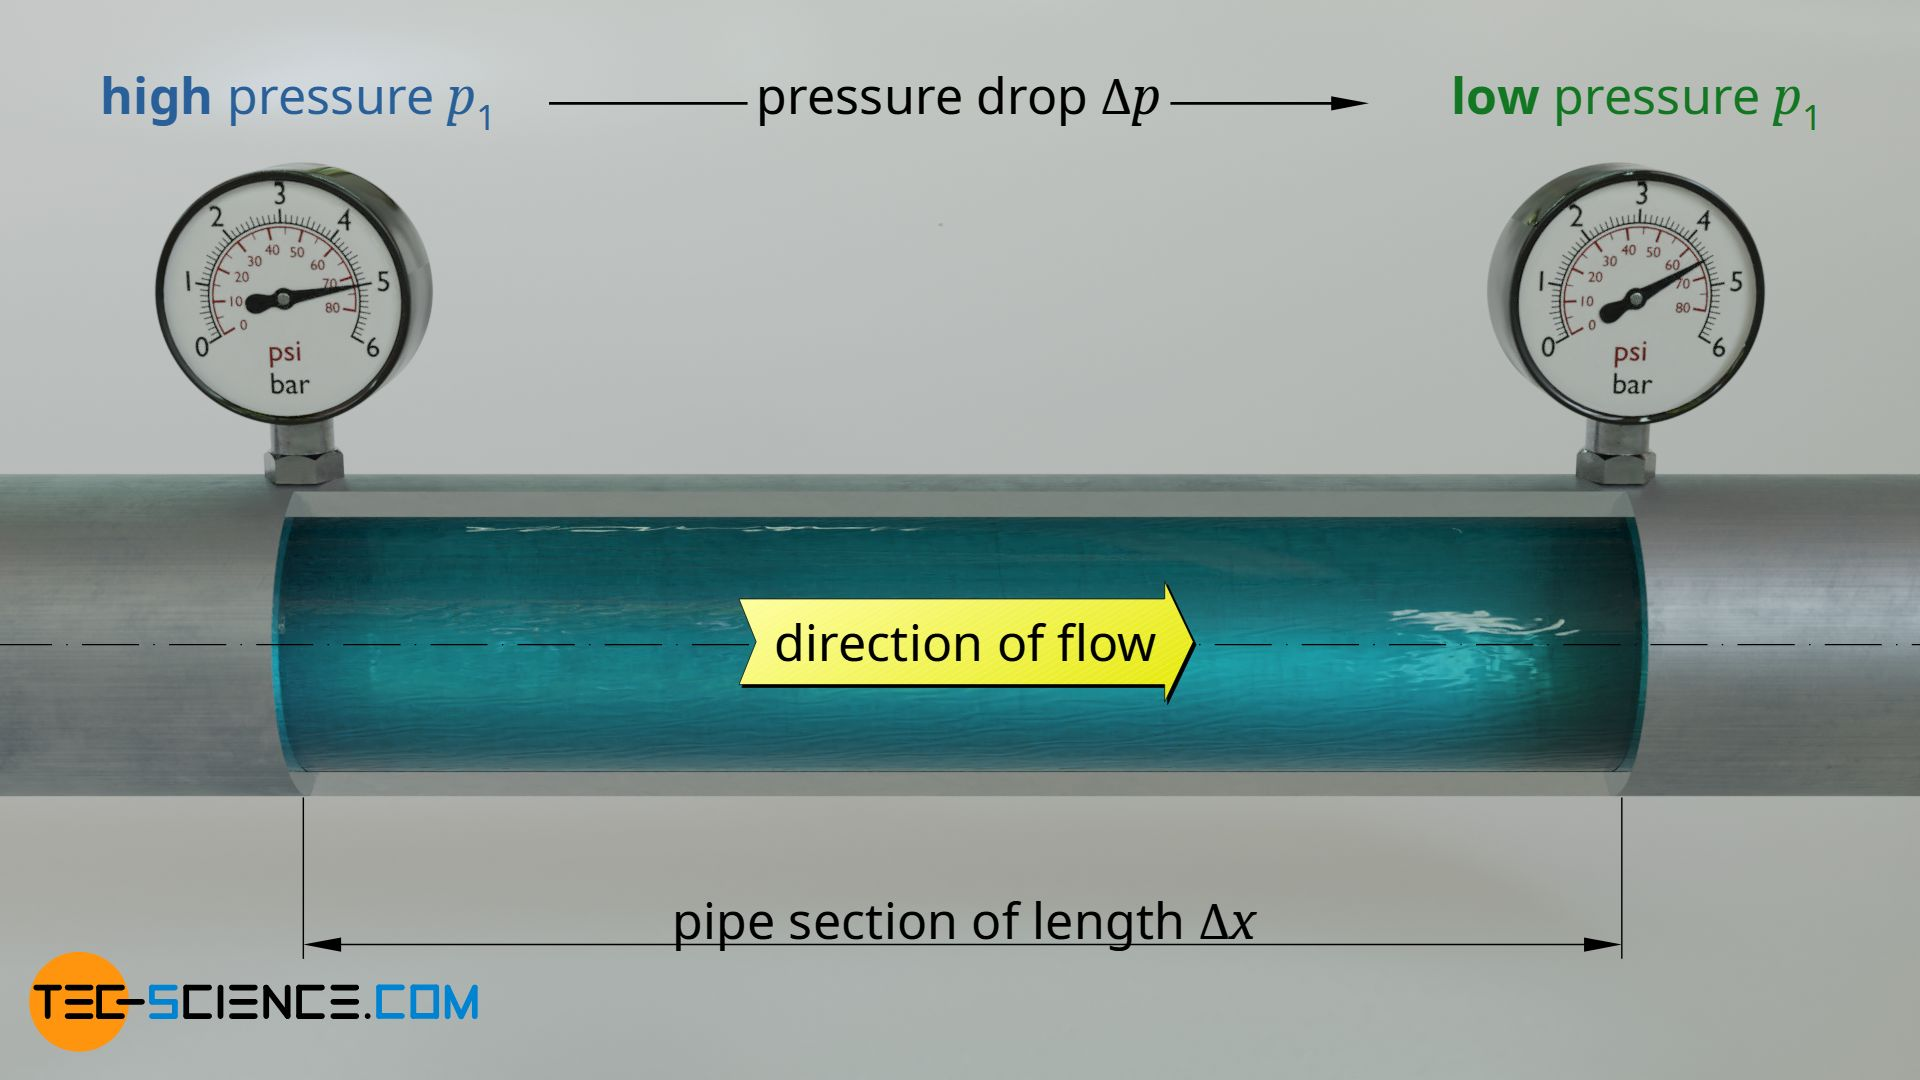
\includegraphics[width=4cm]{../figures/M2/pipe-flow-pressure}}{\footnotesize\par}

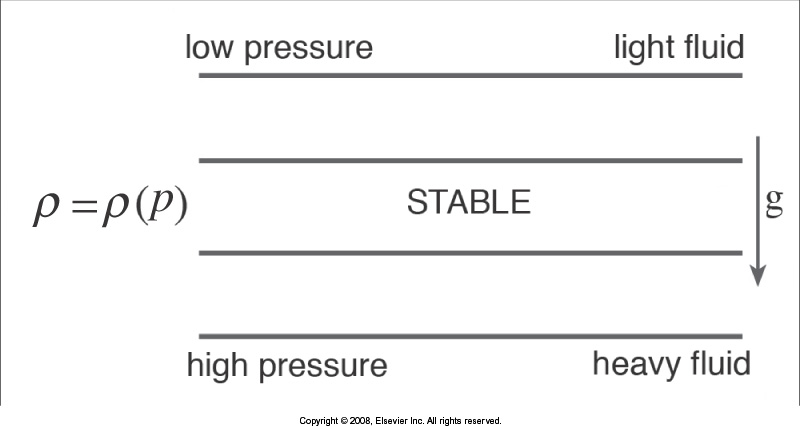
\includegraphics[width=4cm]{../figures/M2/MP-04}

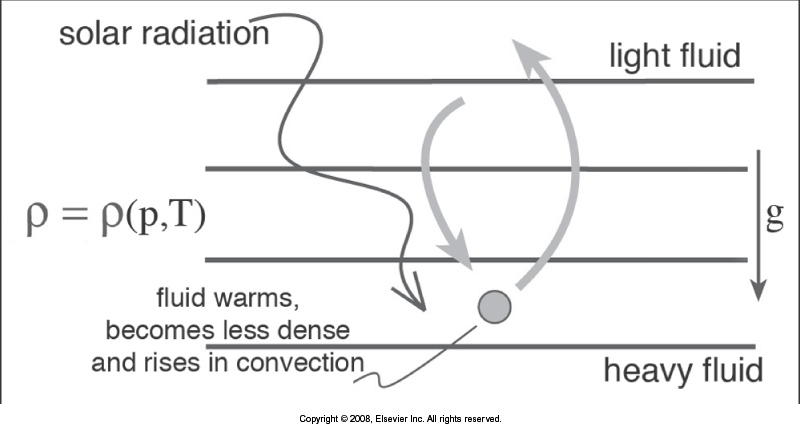
\includegraphics[width=4cm]{../figures/M2/MP-05}
\end{columns}

\end{frame}

\begin{frame}{The vertical thermal structure of natural fluids}

\begin{columns}[t]


\column{6cm}

Standard Atmosphere 40$^{\circ}$N (Dec)

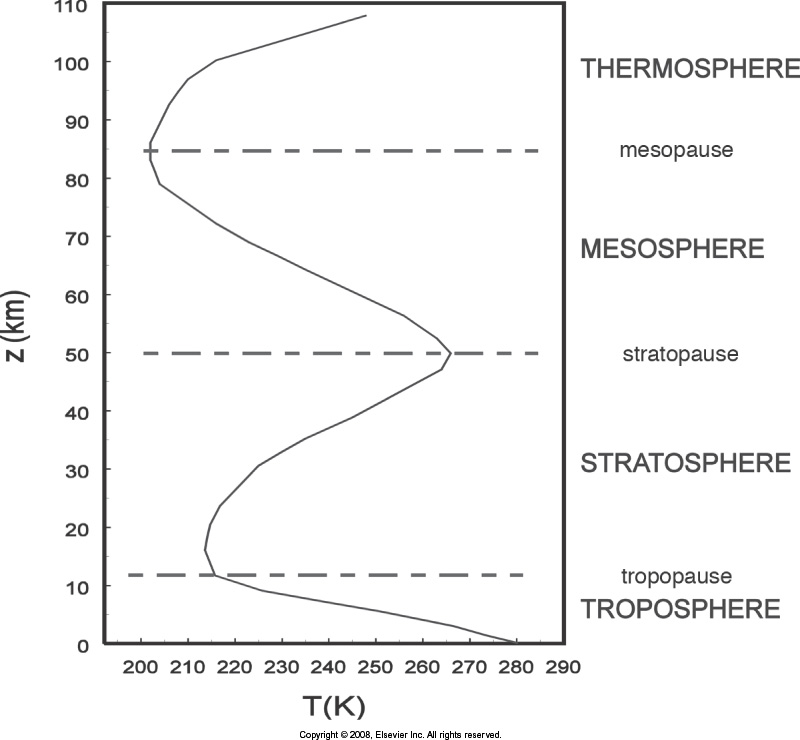
\includegraphics[width=6cm]{../figures/M2/MP-31}

\column{6cm}
\begin{center}
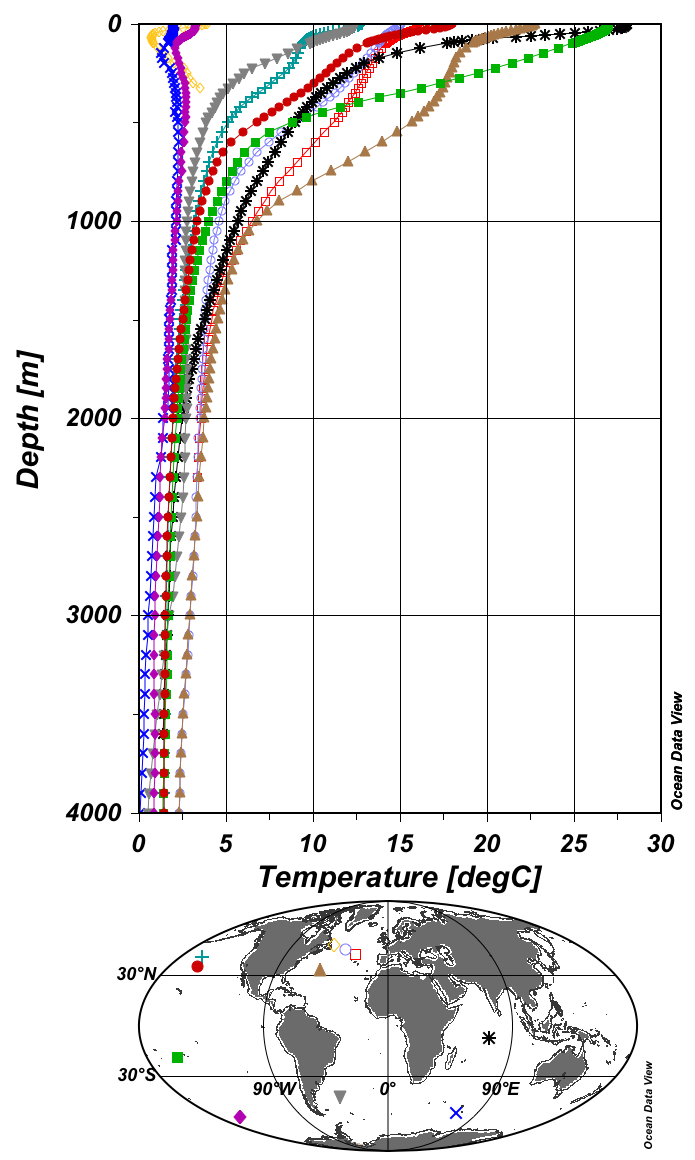
\includegraphics[height=0.8\textheight]{../figures/M2/Temperature_profile_WOA13}
\par\end{center}

\end{columns}

\end{frame}

\begin{frame}{Pressure and density}

\begin{columns}[t]


\column{8cm}
\begin{itemize}
\item {\footnotesize{}Air pressure at a given altitude is the weight of
the air above that level. At (apparent) rest, the fluid is either
homogeneous or stratified: heavier fluid at the bottom, lighter fluid
at the top }{\footnotesize\par}
\item {\footnotesize{}This is a formulation of the }\textbf{\footnotesize{}hydrostatic
balance}{\footnotesize{}, a static equilibrium, which implies that
there is no net acceleration due to pressure or density differences}{\footnotesize\par}
\item {\footnotesize{}The formula can be derived from balancing the forces
acting on a cylinder of air of height $\delta z$ and density $\rho$,
remembering that $p=F/A$. Pressure at the bottom surface is $p_{B}=p(z)$
and pressure at the top is $p_{T}=p(z+\delta z)=p(z)+\delta p$. }\emph{\footnotesize{}Pressure
is identical everywhere at level $z$: note that we do not specify
if the pressure at the top is bigger or smaller, this is what we want
to find out!}{\footnotesize\par}
\end{itemize}

\column{5cm}

\vspace{1cm}
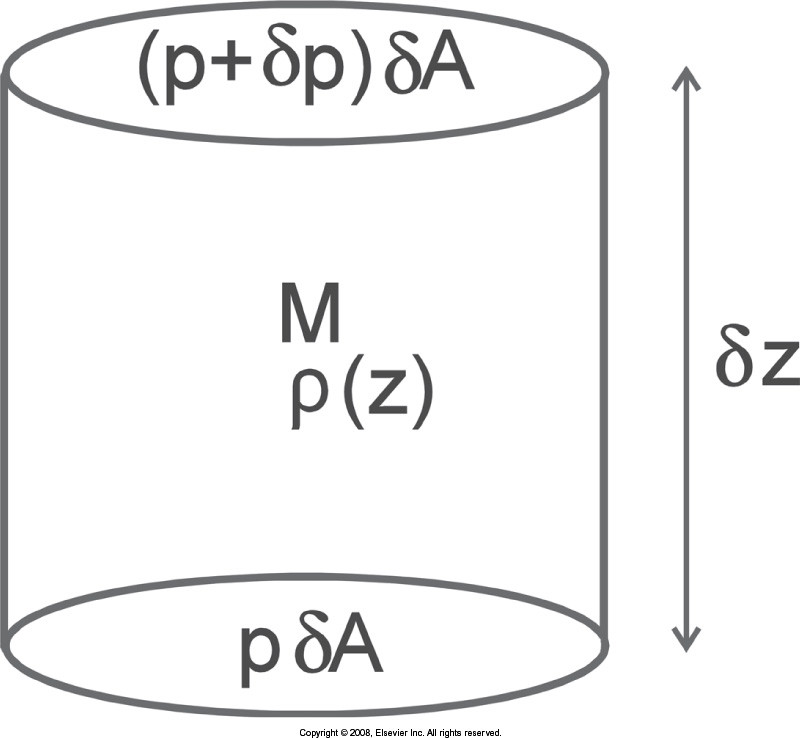
\includegraphics[width=4cm]{../figures/M2/f03-05-P558691}
\end{columns}

\end{frame}

\begin{frame}{The derivation of hydrostatic balance}

\begin{columns}[t]

\column{5cm}
\begin{itemize}
\item {\footnotesize{}The axis $z$ is oriented upward. Looking at the previous
slide, volume and density can be written as follows: $V=\delta A\delta z$;
$\rho=M/V$}{\footnotesize\par}
\item {\footnotesize{}The cylinder is not isolated. There are hypothetical
cylinders all around it, above and below. Remember that pressure is
}\textbf{\footnotesize{}isotropic}{\footnotesize{}, that is, the force
acts in all directions around the cylinder. The pressure forces on
the side will be balancing each other, because the other cylinders
are identical and at the same level.}{\footnotesize\par}
\end{itemize}

\column{7.5cm}
\begin{itemize}
\item {\small{}There are 3 forces acting on the cylinder}

\begin{itemize}
\item {\small{}Gravity: $F_{g}=-gM=-g\rho\delta A\delta z$}{\small\par}
\item {\small{}Pressure at the top: $F_{T}=-p_{T}\delta A$}{\small\par}
\item {\small{}Pressure at the bottom: $F_{B}=p_{B}\delta A$}{\small\par}
\end{itemize}
\item {\small{}No acceleration, so $\sum_{i}F_{i}=F_{g}+F_{T}+F_{B}=0$
\begin{align*}
-g\rho\delta A\delta z-\left(p+\delta p\right)\delta A+p\text{\ensuremath{\delta}A} & =0\\
g\rho\delta z+\delta p & =0\\
\frac{\delta p}{\delta z} & =-\rho g
\end{align*}
}{\small\par}
\end{itemize}
\end{columns}

\end{frame}

\begin{frame}{The hydrostatic balance }

\begin{definition}
Hydrostatic balance describes how pressure decreases with height in
proportion to the weight of the atmosphere above
\[
\frac{\partial p}{\partial z}=-\rho g
\]
\end{definition}

\begin{itemize}
\item The pressure at any height is actually the infinite integral of the
hydrostatic balance, because pressure at infinite height is 0
\[
p(z)=g\int_{z}^{\infty}\rho dz
\]
\item The hydrostatic balance does not tell us how the function $p(z)$
looks like, because we do not know $\rho(z)$. We need a way to compute
the density of a fluid based on its properties. \textbf{We need an
equation of state!}
\end{itemize}
\end{frame}

\begin{frame}{Exercise: compute the mass of the atmosphere}

\begin{itemize}
\item This value is estimated to be $M_{A}=5.26\times10^{18}$ kg
\item Seems impossible to make such a calculation, but it can be estimated
because we can measure the mean surface level pressure (MSLP). 
\item We need to recall that $p=F/A$ and we can use the surface of the
Earth $A_{E}=4\pi a^{2}$
\[
p(z=0)=p_{s}=\frac{gM_{A}}{A_{e}}
\]
\[
M_{A}=\frac{A_{E}p_{s}}{g}
\]
 Find the values on the Internet and check that the number above is
correct.
\end{itemize}
\end{frame}


\section{The equation of state for dry and moist air}
\begin{frame}{Physical properties of air}

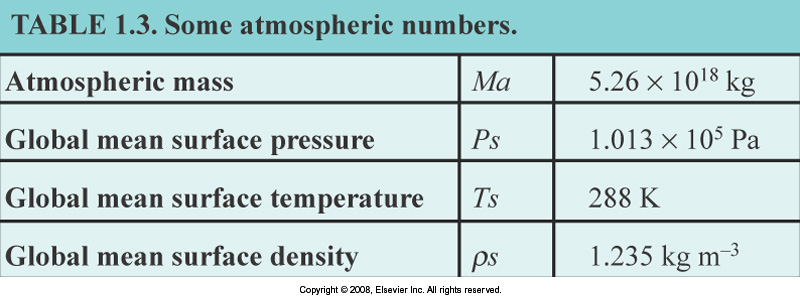
\includegraphics[width=1\paperheight]{../figures/M2/MP_T13}

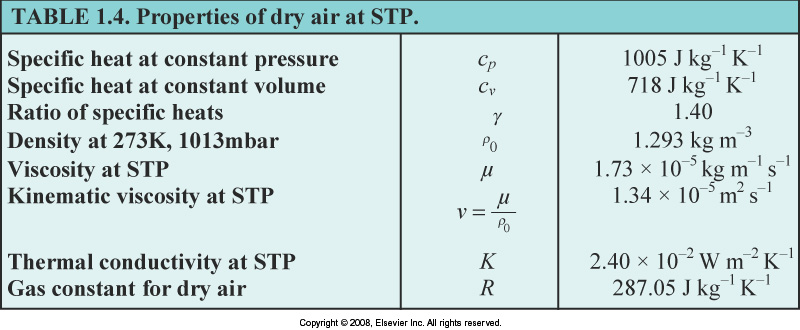
\includegraphics[width=1\paperheight]{../figures/M2/MP_T14}
\end{frame}

\begin{frame}{The equation of state}

\begin{itemize}
\item In mechanics, a material system is decomposed in smaller, meaningful
objects and then their position and velocity are described with dynamical
equations according to the internal and external forces
\item In thermodynamics, the system is described with \uline{ensemble
properties}, based on macroscopic features like temperature or pressure
that are combined to determine a certain state: \textbf{the equation
of state}
\item In the lower atmosphere (up to 50 km) the density of air is sufficiently
high to allow molecules to hit against each other. They can transfer
information and determine locally stable macroscopic mean properties,
a condition called \textbf{local thermodynamic equilibrium} (LTE)
\item Ocean density is much larger and there is LTE everywhere
\end{itemize}
\end{frame}

\begin{frame}{The equation of state for dry air}

\begin{itemize}
\item The dry atmosphere is defined as \textbf{the mixture of gases }\textbf{\emph{excluding
water vapour}}. It follows the perfect gas law
\[
pV=nR_{g}T
\]
where $R_{g}=8.3143$ J K$^{-1}$ mol$^{-1}$ is the universal gas
constant and $n$ is the number of moles of dry air. 
\item In GFD, this equation is usually written in terms of density $\rho=M_{a}/V$
or its inverse, the specific volume $\alpha=V/M_{a}$, where $M_{a}=n\cdot m_{a}$
and $m_{a}=28.97\,10^{-3}$ kg mol$^{-1}$ is the (apparent) molecular
weight of dry air
\item Using the gas constant for dry air $R=R_{g}/m_{a}$ (see Table above),
we obtain the following (equivalent) forms
\[
\boxed{{p\alpha=RT;\ p=\rho RT}}
\]
\end{itemize}
\end{frame}

\begin{frame}{Moist air}

\begin{columns}[t]


\column{8.5cm}

Moist air is dry air + water vapour
\begin{itemize}
\item {\footnotesize{}A mixture of gases follows these principles:}

\begin{itemize}
\item {\footnotesize{}it is possible to use the equation of state for each
single gas}{\footnotesize\par}
\item {\footnotesize{}the pressure of the mixture is given by the sum of
the partial pressures (Dalton's law: the pressure that the gas would
have if it occupied the same volume alone) }{\footnotesize\par}
\end{itemize}
\item {\footnotesize{}By defining $\rho_{v}$ and $\rho_{d}$ the densities
of water vapour and dry air, we have
\begin{align*}
p_{d} & =\rho_{d}R_{d}T;\ e=\rho_{v}R_{v}T\\
p & =p_{d}+e=\left(R_{d}\rho_{d}+R_{v}\rho_{v}\right)T
\end{align*}
}{\footnotesize\par}
\item {\small{}Temperature determines how much water vapour transfers from
liquid to gas phase and ``stay'' in the air}{\small\par}
\end{itemize}

\column{5cm}

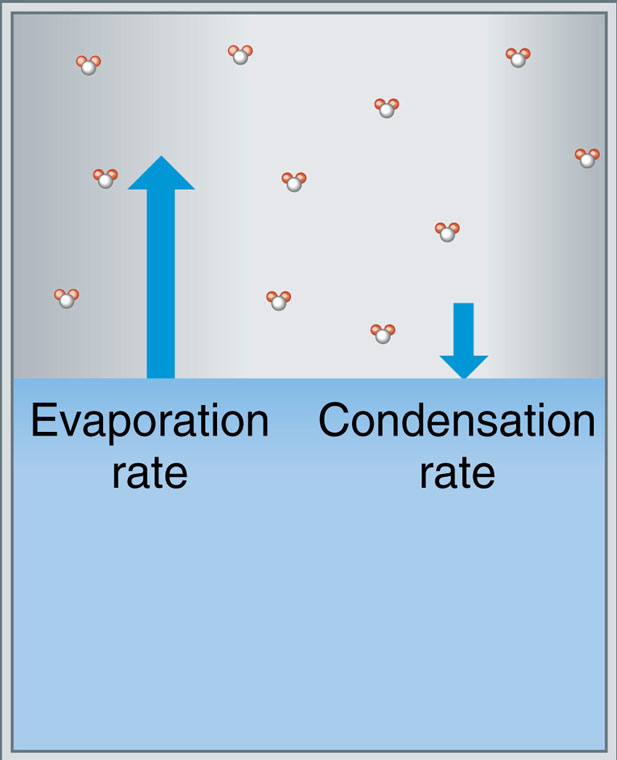
\includegraphics[width=5cm]{../figures/M2/evap_cond}
\end{columns}

\end{frame}

\begin{frame}{Saturation vapour pressure}

\begin{columns}[t]


\column{8.5cm}

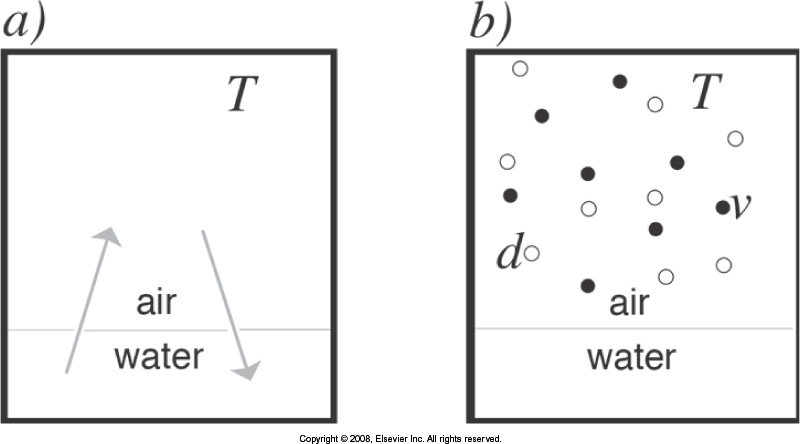
\includegraphics[width=5cm]{../figures/M2/MP_14}
\begin{itemize}
\item {\footnotesize{}The amount of water vapour and its pressure, is a
function of temperature. This principle is stated by the Clausius-Clapeyron
equation (we use a simplified version, A=6.11 hPa; $\beta$=0.067
$^{\circ}$C) 
\[
e_{s}=Ae^{\beta T}
\]
}{\footnotesize\par}
\item {\footnotesize{}Water vapor pressure cannot increase more than a certain
value: there is a balance between evaporation and condensation at
each given temperature. This equilibrium is called }\textbf{\footnotesize{}the
saturation value}{\footnotesize{}. If temperature increases, the saturation
pressure increases, but there cannot be a higher pressure than the
one dictated by this curve }{\footnotesize\par}
\end{itemize}

\column{5cm}

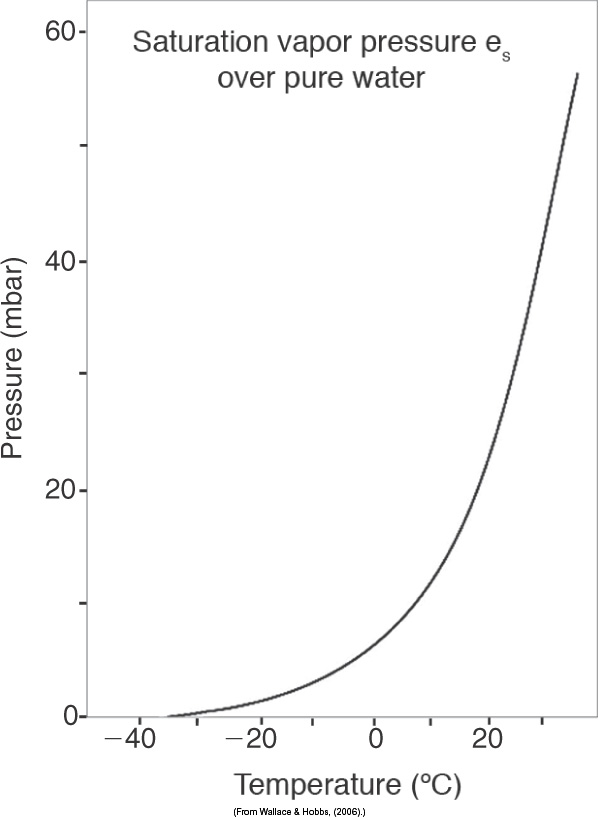
\includegraphics[width=5cm]{../figures/M2/MP_15}
\end{columns}

\end{frame}

\begin{frame}{Specific and relative humidity}

Moisture in the air is defined as the ratio of water vapour mass over
the mass of dry air, the \textbf{mixing ratio} $w=M_{v}/M_{d}=\rho_{v}/\rho_{d}$
(usually in g/kg; in the tropics is 20 g/kg). The more operational
term is however \textbf{humidity}
\begin{definition}
\textbf{\small{}Specific humidity}{\small{} is the ratio of the water
vapour mass to the total mass of air (not much different from the
mixing ratio) 
\[
q=\frac{\rho_{v}}{\rho}=\frac{\rho_{v}}{\rho_{d}+\rho_{v}}
\]
}{\small\par}

\textbf{\small{}Relative humidity}{\small{} is the ratio of specific
humidity to the }\emph{\small{}saturation-specific humidity}{\small{}
(the maximum specific humidity that can be attained in the air at
a given }\emph{\small{}temperature}{\small{} and }\emph{\small{}pressure}{\small{})
\[
RH=\frac{q}{q_{s}}\times100
\]
}{\small\par}
\end{definition}

\end{frame}
%
\begin{frame}{Maximum amount of water in the air}

Relative humidity is the amount of water vapour relative to the maximum
amount of water that can stay in the air at a given temperature. This
latter value is obtained by combining the equation of state for water
vapour with the (simplified) Clausius-Clapeyron equation
\[
\rho_{s}=\frac{e_{s}}{R_{v}T}
\]
\[
e_{S}\approxeq Ae^{\beta T}
\]
\[
\rho_{s}=\frac{Ae^{\beta T}}{R_{v}T};\,\,\,\,q_{s}=\frac{\rho_{s}}{\rho_{d}+\rho_{s}}
\]

\end{frame}

\begin{frame}{Relative humidity and precipitation}

\begin{figure}
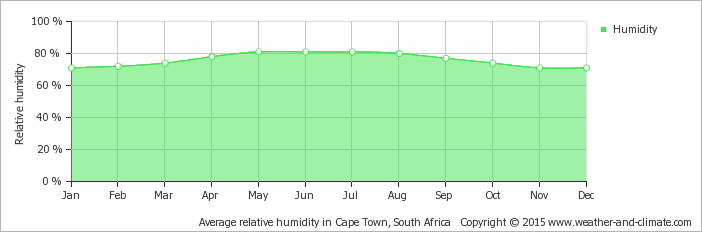
\includegraphics[scale=0.3]{../figures/M2/average-relative-humidity-south-africa-cape_town}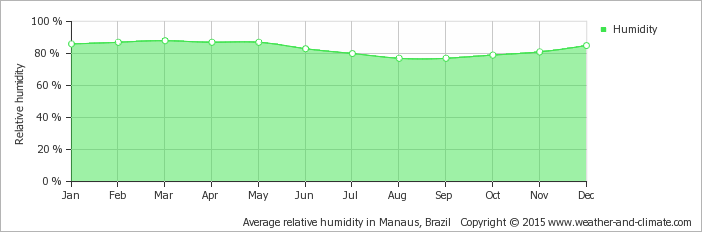
\includegraphics[scale=0.25]{../figures/M2/average-relative-humidity-brazil-manaus}

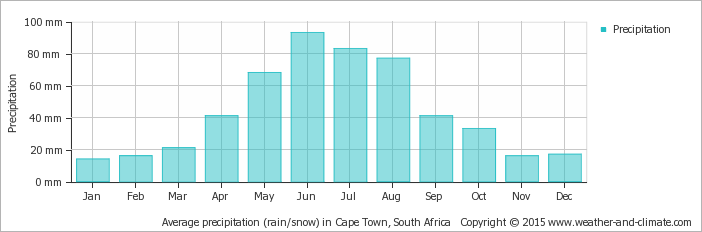
\includegraphics[scale=0.25]{../figures/M2/average-rainfall-south-africa-cape_town}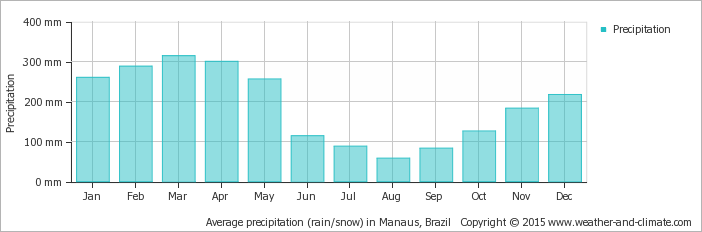
\includegraphics[scale=0.25]{../figures/M2/average-rainfall-brazil-manaus}
\end{figure}
\end{frame}

\begin{frame}{Distribution of water vapour (precipitable water)}

\begin{center}
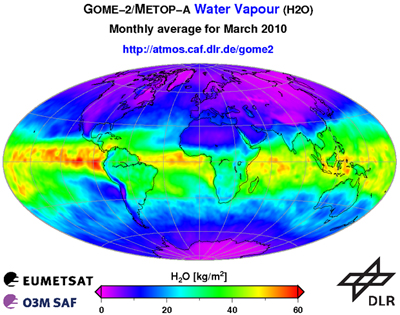
\includegraphics[scale=0.55]{../figures/M2/GOME2_WATER_VAPOUR}
\par\end{center}

\end{frame}

\begin{frame}{Water vapour and climate}


\framesubtitle{\url{http://www.climate.be/textbook/chapter4_node7.html}}
\begin{itemize}
\item Water vapour in the atmosphere has a relevant climatic role: \textbf{it
is an efficient greenhouse gas}
\item The radiative effect of water vapour (the amount of longwave heat
trapped per unit increase of temperature, approx. $\lambda_{v}=1.8\,Wm^{-2}K^{-1}$
\emph{now}) is roughly proportional to the logarithm of the water
vapour concentration, 
\[
\lambda_{v}\propto\log\rho_{v}
\]
and so the influence of an increase in water-vapour content is larger
where the concentration is smaller (think of the derivative of $\log\rho_{v}$)
\item The saturation water vapour (and specific humidity) increases exponentially
with temperature according to Clausius-Clapeyron 
\end{itemize}
\end{frame}

\begin{frame}{Water vapour feedback}


\framesubtitle{\url{http://www.climate.be/textbook/chapter4_node7.html}}
\begin{itemize}
\item A perturbing change in surface temperature, like the one being recorded
in the Earth climate today, is extremely likely, in the absence of
other concurrent feedback, to create an enhancement of the tropospheric
warming
\end{itemize}
\begin{center}
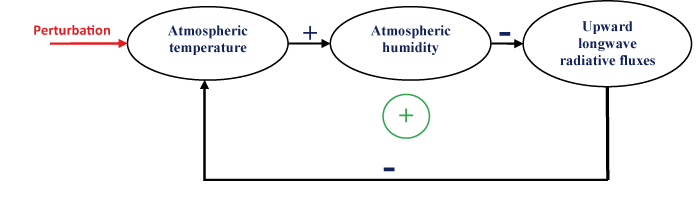
\includegraphics[scale=0.7]{../figures/M2/water_vapour_feedback}
\par\end{center}
\begin{itemize}
\item {\footnotesize{}This is a simple form of the water vapour feedback,
where the symbol $+$ indicates a direct relationship (both components
increase or decrease together), the symbol $-$ indicates inverse
relationship (if one component increases, the other decreases or viceversa).
Feedbacks signs combine like in algebra to get the final sign.}{\footnotesize\par}
\end{itemize}
\end{frame}

\begin{frame}{Exercise 1}

\begin{itemize}
\item \textbf{Calculate the density of water vapour that exerts a pressure
of 9 mb at 20$^{\circ}C$}
\item Take the equation of state for water vapour $e=\rho_{v}R_{v}T$ and
first compute its gas constant from the universal gas constant $R_{g}=8.3143$
J K$^{-1}$ mol$^{-1}$ and the molecular weight of water ($m_{a}=18.016\,10^{-3}$
kg mol$^{-1}$)
\[
R_{v}=\frac{R_{g}}{m_{v}}=\frac{8.3143}{18.016\,10^{-3}}=461\ J\,kg^{-1}\,K^{-1}
\]
\item Remember that we work with the SI and \textbf{mb} \textbf{is not}
SI units: 9 mb = 9 hPa = 900 Pa; temperature must be converted to
kelvin units, 20\textbf{$^{\circ}C$ }= 293.15 K
\[
\rho_{v}=\frac{e}{R_{v}T}=\frac{900}{461\cdot293.15}=0.006659654297345=6.66\,10^{-3}\,kg\,m^{-3}
\]
\end{itemize}
\end{frame}

\begin{frame}{Exercise 2}

\begin{itemize}
\item \textbf{\small{}If air contains water vapour with a mixing ratio of
5.5 g/kg and the total pressure is 1026.8 hPa, calculate the vapour
pressure with 1 significant figure}{\small\par}
\item {\small{}We don't know the temperature, so cannot apply the equation
of state. We know the Dalton's law that says total pressure is the
sum of the pressure of dry air and the water vapour pressure, and
pressure will depend on the number of moles of each gas 
\begin{align*}
p & =p_{d}+e=\frac{n_{d}}{n_{d}+n_{v}}p+\frac{n_{v}}{n_{d}+n_{v}}p\\
e & =\frac{n_{v}}{n_{d}+n_{v}}p=\frac{\frac{M_{v}}{m_{v}}}{\frac{M_{d}}{m_{d}}+\frac{M_{v}}{m_{v}}}p
\end{align*}
}{\small\par}
\item {\small{}we know the mixing ratio $w=M_{v}/M_{d}$ and we need to
put it in the equation, so if we multiply by $m_{v}/M_{d}$ both numerator
and denominator we get
\[
e=\frac{\frac{M_{v}}{M_{d}}}{\frac{m_{v}}{m_{d}}+\frac{M_{v}}{M_{d}}}p=\frac{w}{\varepsilon+w}p=\frac{5.5\,10^{-3}}{0.622+5.5\,10^{-3}}1026.8=8.99984=9\,hPa
\]
}{\small\par}
\end{itemize}
\end{frame}


\section{The equation of state for seawater}
\begin{frame}{Physical properties of seawater}

\begin{columns}[t]


\column{7cm}
\begin{itemize}
\item The mean density of seawater is slightly higher than fresh water (on
average $1.035\:10^{3}$ kg m$^{-3}$) and, unlike air density, it
varies very little. Because of these tiny but dynamically significant
variations, the density of seawater has been expressed in several
ways 
\item Seawater density depends on temperature, salinity and pressure in
a complicated way that requires careful laboratory measurements
\end{itemize}

\column{6.5cm}

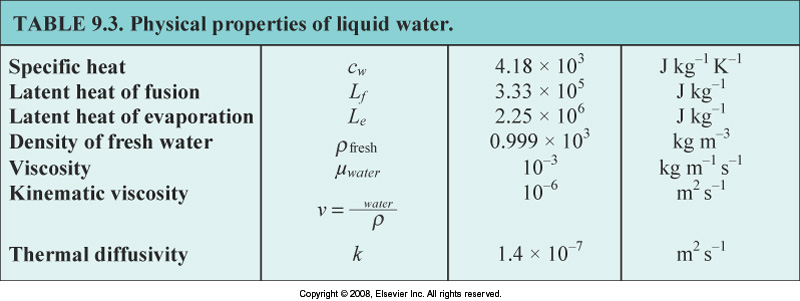
\includegraphics[width=6.6cm]{../figures/M2/MP_T93.jpg}
\begin{itemize}
\item Seawater density is $\rho=\rho\left(T,S,p\right)$ but there is no
``perfect'' equation of state for it. We instead use the \textbf{Thermodynamic
Equation Of Seawater} - 2010 (TEOS-10, \url{http://www.teos-10.org/})
\end{itemize}
\end{columns}

\end{frame}

\begin{frame}{Notations for density}

\begin{itemize}
\item Density definition depends on 

\begin{enumerate}
\item the choice of the reference level
\item the effects of pressure
\end{enumerate}
\item In situ density $\rho$ 
\item \textbf{Density anomaly} $\sigma=\rho-\rho_{ref}=\rho-1000$ (note
that the reference is an arbitrary value)
\item Potential density anomaly $\sigma_{\theta}$ (related to potential
temperature $\theta$) 
\item Density anomalies at reference surfaces are computed using the mean
density from that surface: $\sigma_{t}$ (0 m), $\sigma_{2}$ (2000
m), $\sigma_{4}$ (4000 m), etc.
\end{itemize}
\end{frame}

\begin{frame}{Effects of T, S and p}

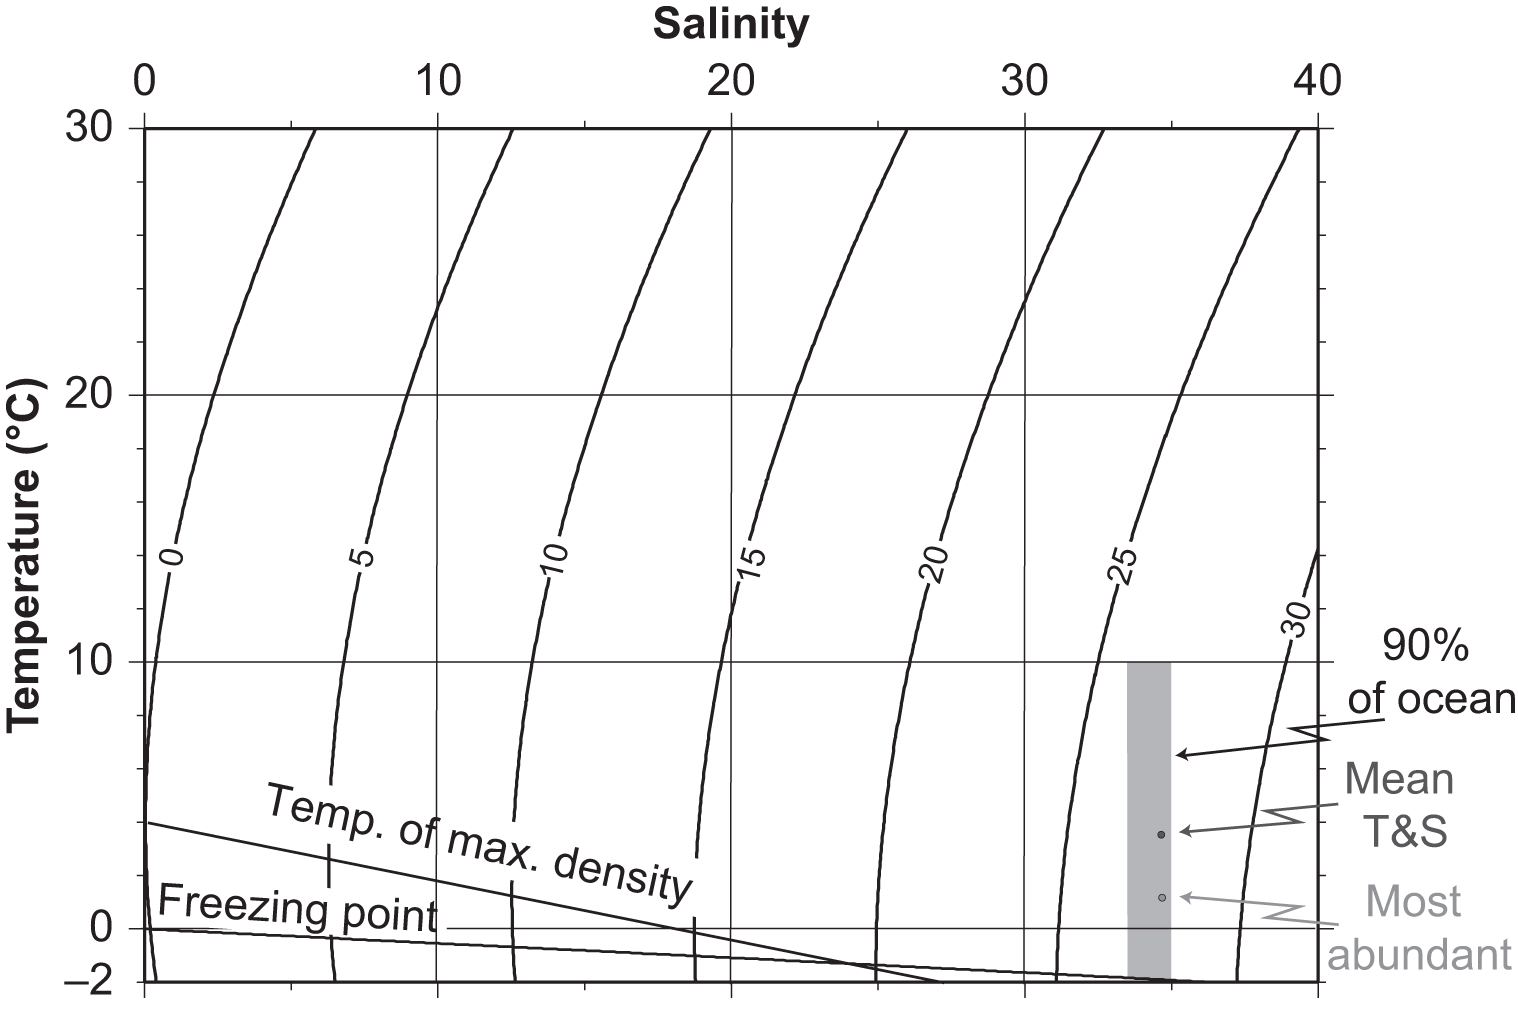
\includegraphics[width=7cm]{../figures/M2/T-31.jpg}
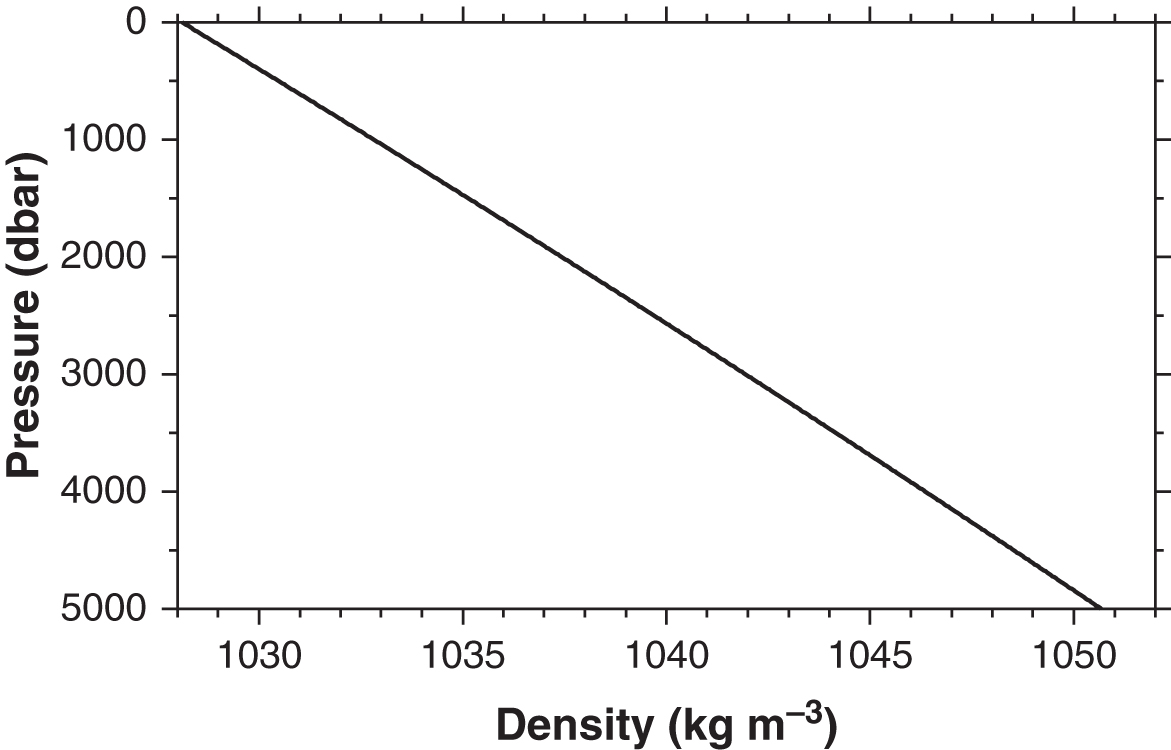
\includegraphics[width=6cm]{../figures/M2/T-34.jpg}

Dependence of density anomaly (left) on T and S and in situ density
on pressure (right, from Talley et al.). See also figure 9.2 M\&P
\end{frame}

\begin{frame}{The ``linear'' equation of state for seawater}

\begin{columns}[t]


\column{12cm}
\begin{itemize}
\item {\tiny{}In the narrow range of T and S found in the ocean, temperature
influences density much more than salinity, because there are much
larger changes (we ignore pressure for now). The differential of the
density equation, is written as
\[
d\rho=\frac{\partial\rho}{\partial T}dT+\frac{\partial\rho}{\partial S}dS;\:\rho=\rho\left(T,S\right)
\]
}{\tiny\par}
\item {\tiny{}The thermal expansion coefficient is not a constant and depends
on temperature and pressure (and salinity). The mean value is $10^{-4}$
K$^{-1}$ and it is defined as 
\[
\alpha_{T}=-\frac{1}{\rho_{ref}}\frac{\partial\rho}{\partial T}
\]
}{\tiny\par}
\item {\tiny{}The haline contraction coefficient gives the change in density
per units salinity and has a mean value of $7.7\times10^{-4}$ psu$^{-1}$
(note, this is done using the practical salinity scale, PSS-78), 
\[
\beta_{S}=\frac{1}{\rho_{ref}}\frac{\partial\rho}{\partial S_{P}}
\]
}{\tiny\par}
\item {\tiny{}The approximated linear equation of state is a Taylor expansion
around $\sigma_{0}(T_{0},S_{0})$
\[
\sigma=\sigma_{0}+\rho_{ref}\left[-\alpha_{T}\left(T-T_{0}\right)+\beta_{S}\left(S-S_{0}\right)\right]
\]
}{\tiny\par}
\end{itemize}

\column{4cm}

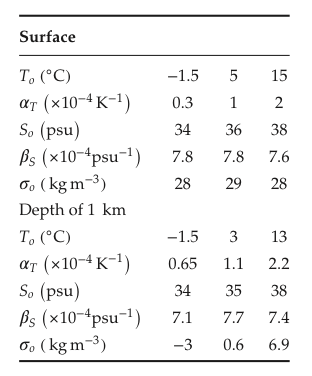
\includegraphics[width=4cm]{../figures/M2/MP_T94.png}
\end{columns}

\end{frame}

\begin{frame}{TEOS-10}

\begin{itemize}
\item The 1980 International Equation of State (EOS-80), which used the
practical salinity scale PSS-78, has served the community very well
for 30 years. 
\item EOS-80 provides separate algorithms for density, sound speed, heat
capacity and freezing temperature. 
\item However, EOS-80 does not provide expressions for entropy, internal
energy and most importantly enthalpy (a measure of the internal energy
of a substance). The real density is based on two major properties:
\textbf{Absolute Salinity} and \textbf{Conservative Temperature}.
\item The TEOS-10 (Thermodynamic Equation Of Seawater -- 2010) \emph{Gibbs}
function incorporates the most recent laboratory data, making the
algorithms more accurate, e. g. - the properties of pure water are
more accurate than in EOS-80, - the temperature scale has been updated
from IPTS-68 to ITS-90. - the density of very cold brackish water
is significantly improved. 
\end{itemize}
\end{frame}

\begin{frame}{Absolute Salinity}

\begin{itemize}
\item \textbf{Practical Salinity} (PSS-78) is calculated from the conductivity
of seawater. \textbf{It is not the mass fraction of salt in seawater}
\item $S_{\mathrm{P}}$ reflects the conductivity of seawater whereas the
thermodynamic properties are better expressed in terms of the concentrations
of all the soluble components. For example, non-ionic species contribute
to density but not to conductivity. 
\item \textbf{Absolute Salinity} $S_{\mathrm{A}}$ is related to Practical
Salinity $S_{\mathrm{P}}$ (which is based on conductivity ratio)
and the \textbf{Absolute Salinity anomaly} 
\[
S_{\mathrm{A}}=\frac{35.16504}{35}\left[g/kg\right]\times S_{\mathrm{P}}+\delta S_{\mathrm{A}}\left(x,y,p\right)
\]
\item The density of seawater is a function of $S_{A}$ not of $S_{P}$.
Only Absolute Salinity can accurately determine the horizontal density
gradients that drive the motion of geophysical fluids (the \textquotedblleft thermal
wind\textquotedblright{} equation used to derive fluid velocities,
which we will see later on in the course)
\end{itemize}
\end{frame}

\begin{frame}{How do we know the values of Absolute Salinity anomaly?}

\begin{columns}[t]


\column{7cm}
\begin{itemize}
\item {\small{}Determined by accurately measuring the density of a seawater
sample in the laboratory and comparing to $\rho\left(T,S_{\mathrm{P}},p\right)$}{\small\par}
\item {\small{}Done this to date on 811 seawater samples (growing) from
around the global ocean and then interpolated}{\small\par}
\end{itemize}
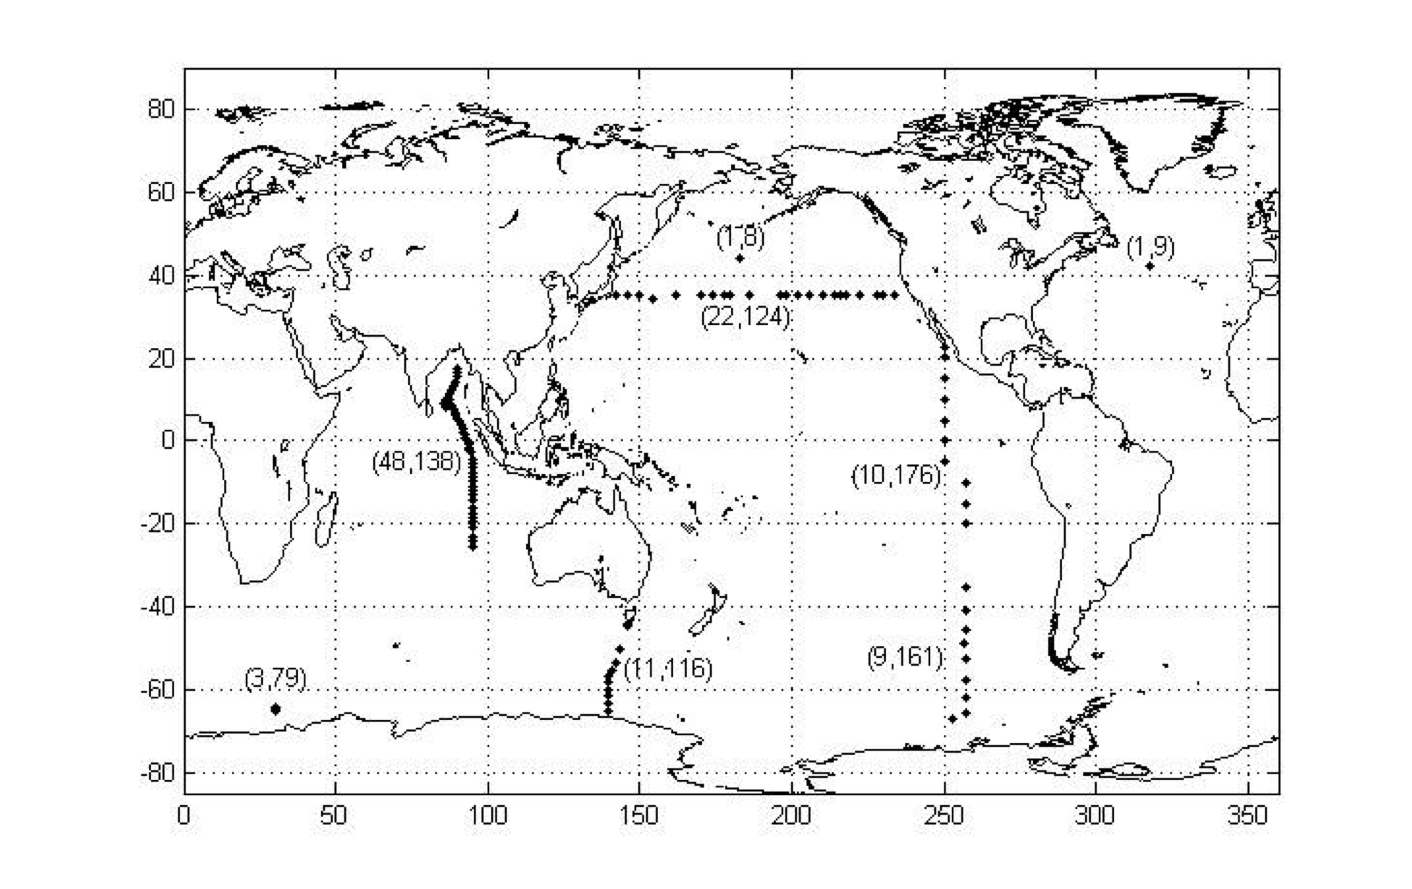
\includegraphics[width=6cm]{../figures/M2/deltaSA_samples.png}

\column{6cm}

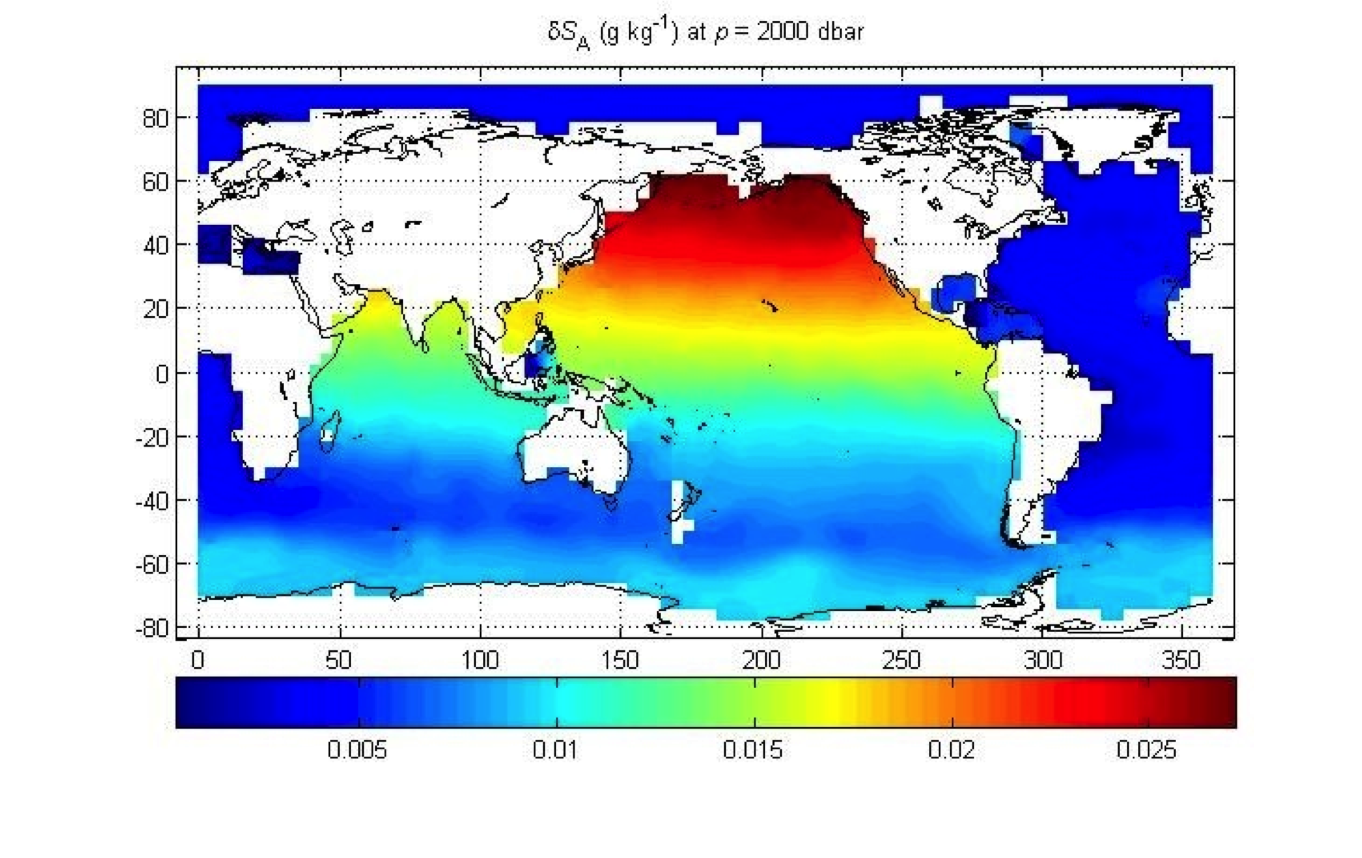
\includegraphics[width=5.5cm]{../figures/M2/deltaSA_field.png}

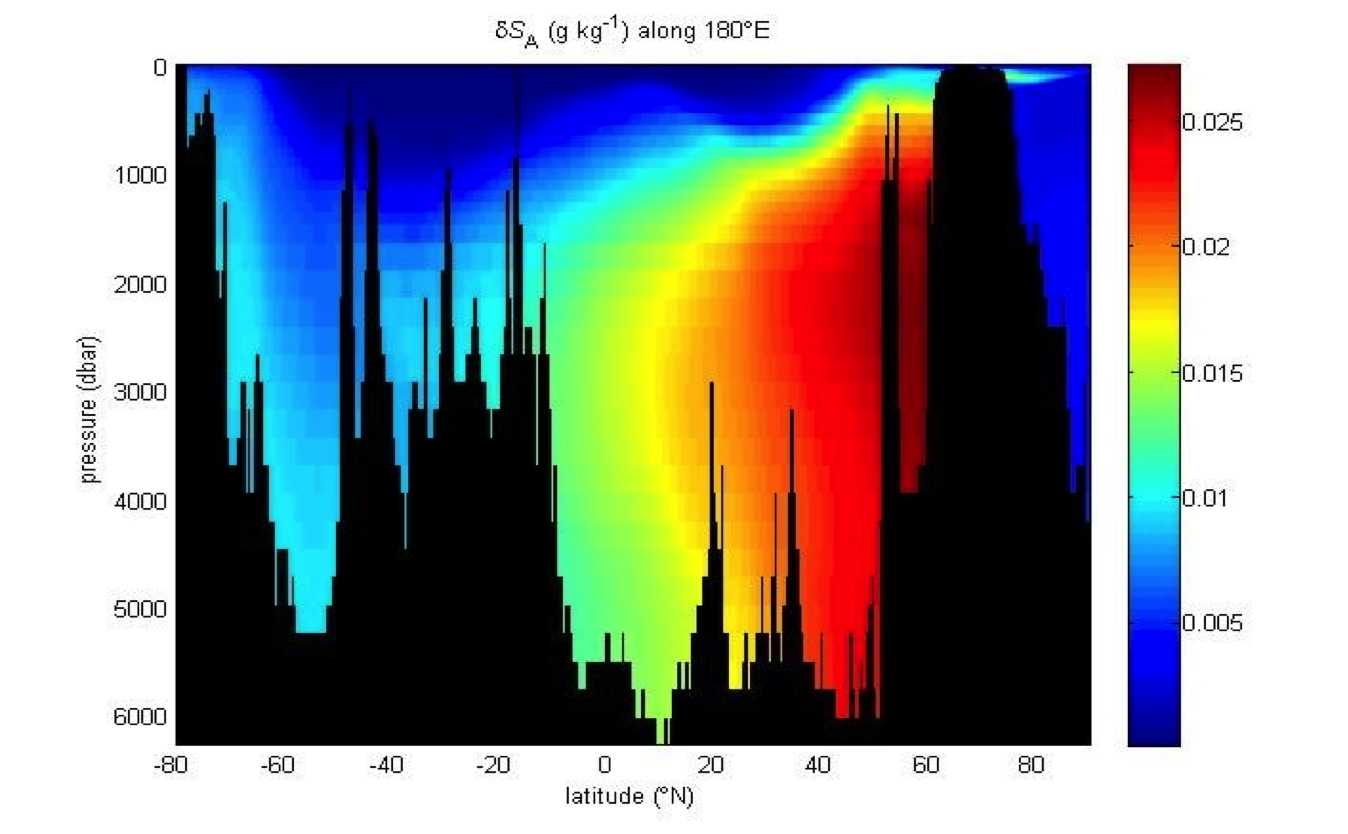
\includegraphics[width=5.5cm]{../figures/M2/deltaSA_section.png}
\end{columns}

\end{frame}

\begin{frame}{Potential temperature\footnote{Seawater properties and potential temperature are revised in the supplementary
material on Vula (Lecture notes by B Loveday. It is part of the study
material and it will be in the quizzes)}}


\framesubtitle{from TJ McDougall Introduction to TEOS-10}
\begin{itemize}
\item \textbf{Potential temperature} $\theta$ involves a \textbf{thought
experiment} and it is a practical way to approximate processes when
making derivations (potential temperature is the basic state variable
in atmospheric dynamics, because it can be derived using an exact
equation of state). 
\item It is the temperature that a parcel of water \emph{``had if it was
at the surface''} . You take a seawater sample at pressure $p$ (at
a given in situ $T)$ and you mentally put an insulating bag around
it (\textbf{adiabatic process}), and then you change its pressure
while taking it towards the surface. Once there, you \textquotedblleft measure\textquotedblright{}
the resulting temperature. 
\item Potential temperature and \emph{in situ} temperature are identical
for samples measured at the surface, but they differ at depth due
to the effect of pressure
\end{itemize}
\end{frame}

\begin{frame}{Conservative temperature and the true density of seawater}

\begin{columns}[t]


\column{9.5cm}
\begin{itemize}
\item {\small{}Just as potential temperature $\theta$ is the temperature
evaluated after an adiabatic change in pressure, so }\textbf{\small{}potential
enthalpy}{\small{} is the enthalpy of a fluid parcel after the same
adiabatic change in pressure}{\small\par}
\item {\small{}The first law of thermodynamic can be written in terms of
a }\textbf{\small{}Conservative Temperature}{\small{} $\Theta$, which
is expressed using a constant specific heat $\left(h^{0}=c_{p}^{0}\Theta\right)$}{\small\par}
\item {\small{}This is a polynomial expression, computed with high quality
software (MATLAB, C, FORTRAN and python \url{http://www.teos-10.org/})}{\small\par}
\item \textbf{The use of $S_{A}$ and $\Theta$ will give you the true density
of seawater. }\textbf{\emph{Note that for historical continuity, data
records are still stored with in situ and practical salinity units.}}
\end{itemize}

\column{6.5cm}

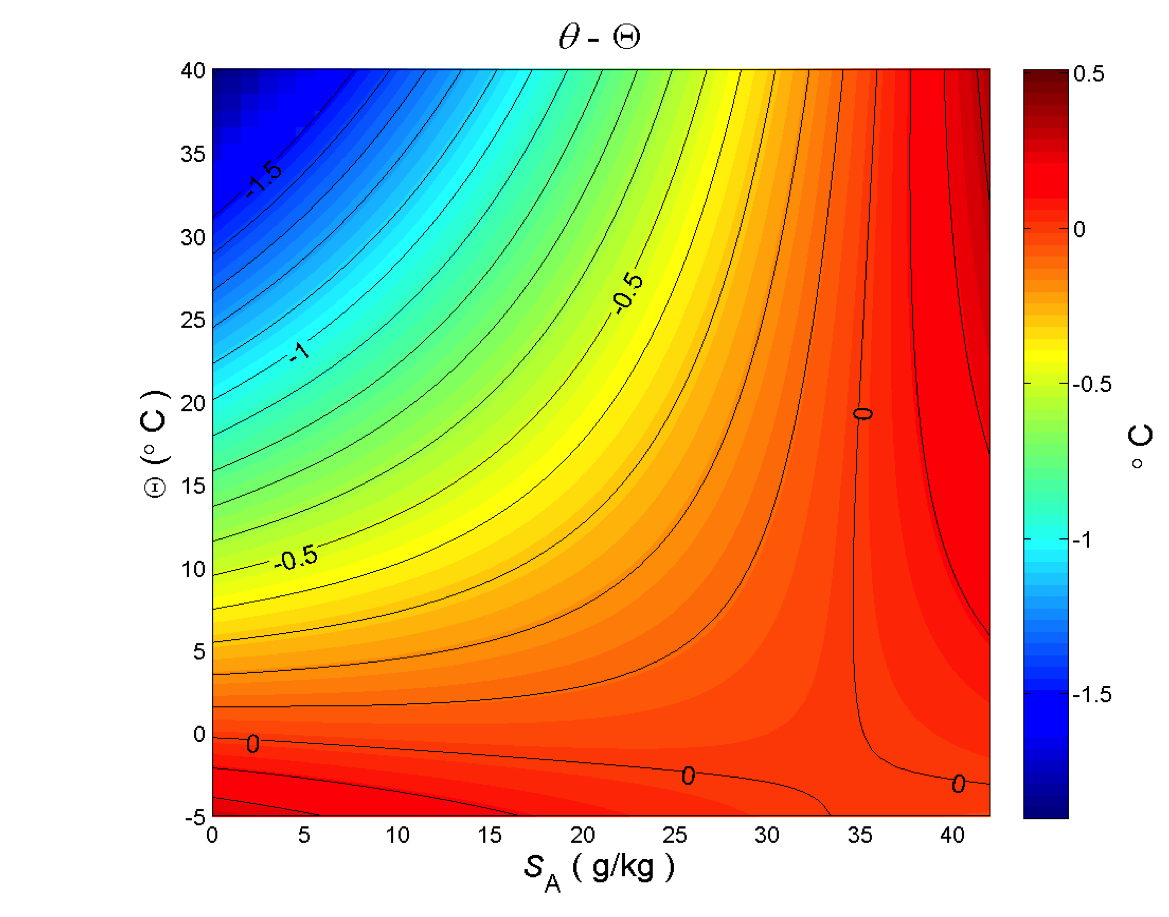
\includegraphics[width=6.6cm]{../figures/M2/conservative_temp.png}
\end{columns}

\end{frame}

\section{Vertical structure of pressure and density in the atmosphere}
\begin{frame}{Vertical structure of pressure}

\begin{columns}[t]


\column{4cm}

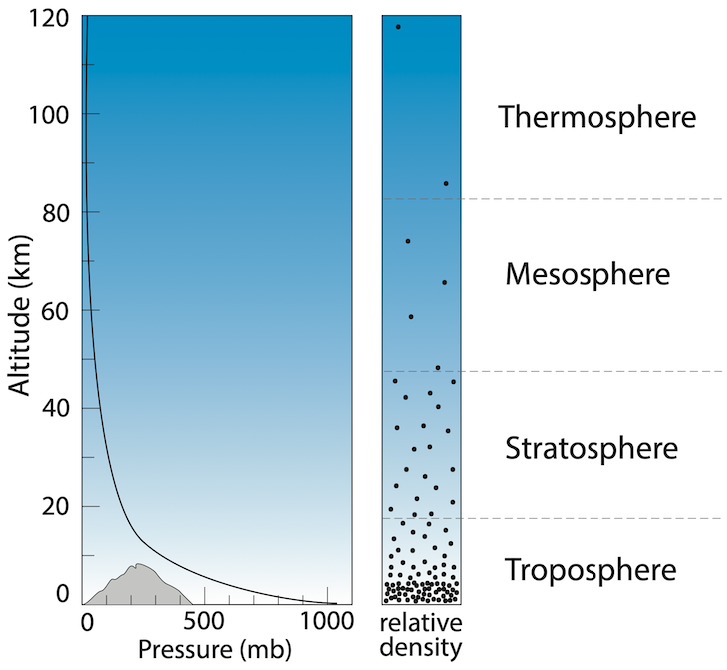
\includegraphics[width=5cm]{../figures/M2/pressure-vs-altitude}

\column{10cm}
\begin{itemize}
\item \label{frame:vertical-structure-pressure}We can \textbf{combine together
the equation of state} for the atmosphere $\left(p=\rho RT\right)$
\textbf{and the hydrostatic balance equation} $\left(\partial p/\partial z=-\rho g\right)$
to obtain a function of how pressure varies with height
\[
\frac{\partial p}{\partial z}=-g\frac{p}{RT}
\]
\item This is not really helpful because we have just added another variable
$T(z)$. However, the vertical thermal structure in the troposphere
is quite constrained around 240-250 K. We can derive some interesting
features of the pressure field by assuming that temperature is constant
with height
\end{itemize}
\end{columns}

\end{frame}

\begin{frame}{Theory and observations}

\begin{columns}[t]


\column{7cm}
\begin{itemize}
\item Observed profile of pressure (solid) plotted against the theoretical
profile (dashed) obtained with the equation of an \textbf{isothermal
atmosphere} 
\item Note that the scale is logarithmic
\end{itemize}

\column{6cm}

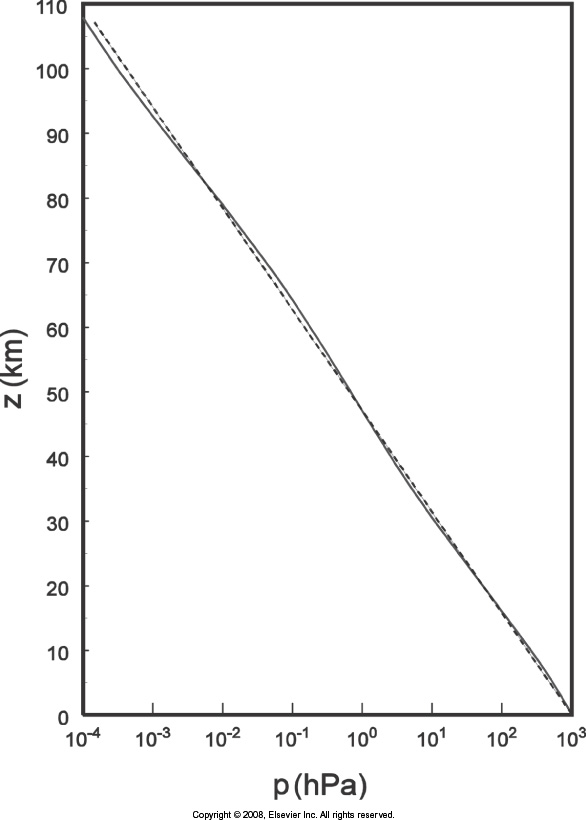
\includegraphics[width=5cm]{../figures/M2/f03-06-P558691}
\end{columns}

\end{frame}

\begin{frame}{Pressure in an isothermal atmosphere}

\begin{itemize}
\item {\small{}In an isothermal atmosphere we assume that $T=T_{0}$ (and
also that $g$ does not change much with height). The hydrostatic
balance equation is simplified to contain one }\textbf{\small{}dependent
variable}{\small{} (pressure) and one }\textbf{\small{}independent
variable}{\small{} (height)
\[
\frac{\partial p}{\partial z}=-\frac{gp}{RT_{0}}=-\frac{p\left(z\right)}{H}
\]
}{\small\par}
\item {\small{}We have defined the constant $H=RT_{0}/g$ called the }\textbf{\small{}scale
height}{\small{}. This is an }\textbf{\small{}ordinary differential
equation}{\small{} that can be solved by separation of variables considering
the boundary condition $p(z=0)=p_{s}$: 
\[
\boxed{p(z)=p_{s}e^{-\frac{z}{H}}}
\]
}\textbf{\small{}Pressure decreases with height with an e-folding
scale $H$ starting from the surface pressure value. }\emph{\small{}Before
proceeding, compute the value of H on your own and check the units
(use a temperature value of 250 K).}{\small\par}
\end{itemize}
\end{frame}
%
\begin{frame}{The scale height and the standard atmosphere}

\begin{columns}[t]


\column{9cm}
\begin{itemize}
\item {\footnotesize{}The scale height is a measure of how pressure (and
density) decreases with height. The }\textbf{\footnotesize{}US standard
atmosphere}{\footnotesize{} (1976) is an idealised function that has
been proposed as the reference atmosphere where the scale height is
similar to observations of pressure changes with height}{\footnotesize\par}
\item {\footnotesize{}Temperature varies linearly within the layers, so
$H(z)=RT(z)/g$ is linear as well}{\footnotesize\par}
\item {\footnotesize{}Much can be done by assuming a constant $T$, like
T=250 K in the troposphere. Using $R=287.05$ J kg$^{-1}$ K$^{-1}$,
the scale height is about $H=7.32$ km}{\footnotesize\par}
\item {\footnotesize{}The engineered equations of the standard atmosphere
are used in aeronautics and meteorological applications}{\footnotesize\par}
\end{itemize}

\column{6cm}

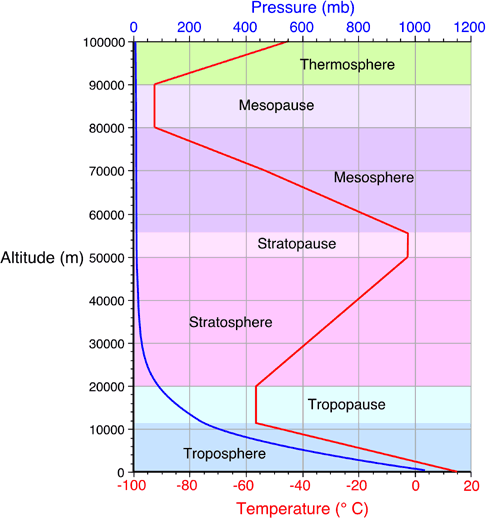
\includegraphics[width=6cm]{../figures/M2/atmslayers}
\end{columns}

\end{frame}

\begin{frame}{Density in an isothermal atmosphere}

\begin{itemize}
\item {\small{}Let's combine the equation above, $p(z)=p_{s}e^{-\frac{z}{H}}$
with the equation of state $p=\rho RT_{0}$ to further derive the
change in density with height 
\[
\boxed{\rho(z)=\frac{p_{s}}{RT_{0}}e^{-\frac{z}{H}}=\rho_{0}e^{-\frac{z}{H}}}
\]
}{\small\par}
\item {\small{}This equation can be used: }{\small\par}
\begin{enumerate}
\item {\small{}to compute the percentage or fraction of air (wrt the surface
density) found at a given altitude (e.g. the troposphere $Z_{tropo}=10^{4}$
m)
\[
\rho/\rho_{0}=e^{-\frac{Z_{tropo}}{H}}
\]
}{\small\par}
\item {\small{}to compute the height at which density has decreased of a
given percentage
\[
\ln\rho/\rho_{0}=\ln e^{-\frac{z}{H}}
\]
\[
z=-H\ln\rho/\rho_{0}
\]
}{\small\par}
\end{enumerate}
\end{itemize}
\end{frame}


\section{Geopotential height}
\begin{frame}{Pressure as indicator of air mass features}

\begin{columns}[t]

\column{7cm}
\begin{itemize}
\item {\footnotesize{}In hydrostatic balance, pressure is directly related
to the overlying amount of air. Pressure is thus an indicator of mass
in the atmosphere, whose density is linked to temperature. }{\footnotesize\par}
\item {\footnotesize{}In observations, }\textbf{\footnotesize{}it is simpler
to measure pressure }\textbf{\emph{\footnotesize{}in situ}}\textbf{\footnotesize{}
rather than height}{\footnotesize{} both in the atmosphere and in
the ocean. In atmospheric sciences surface }\textbf{\footnotesize{}pressure
levels}{\footnotesize{} become the reference system of coordinates.}{\footnotesize\par}
\item {\footnotesize{}The thickness of the air layer between two pressure
levels (called isobars) is an }\textbf{\footnotesize{}indication of
the layer's temperature}{\footnotesize\par}
\end{itemize}

\column{7cm}

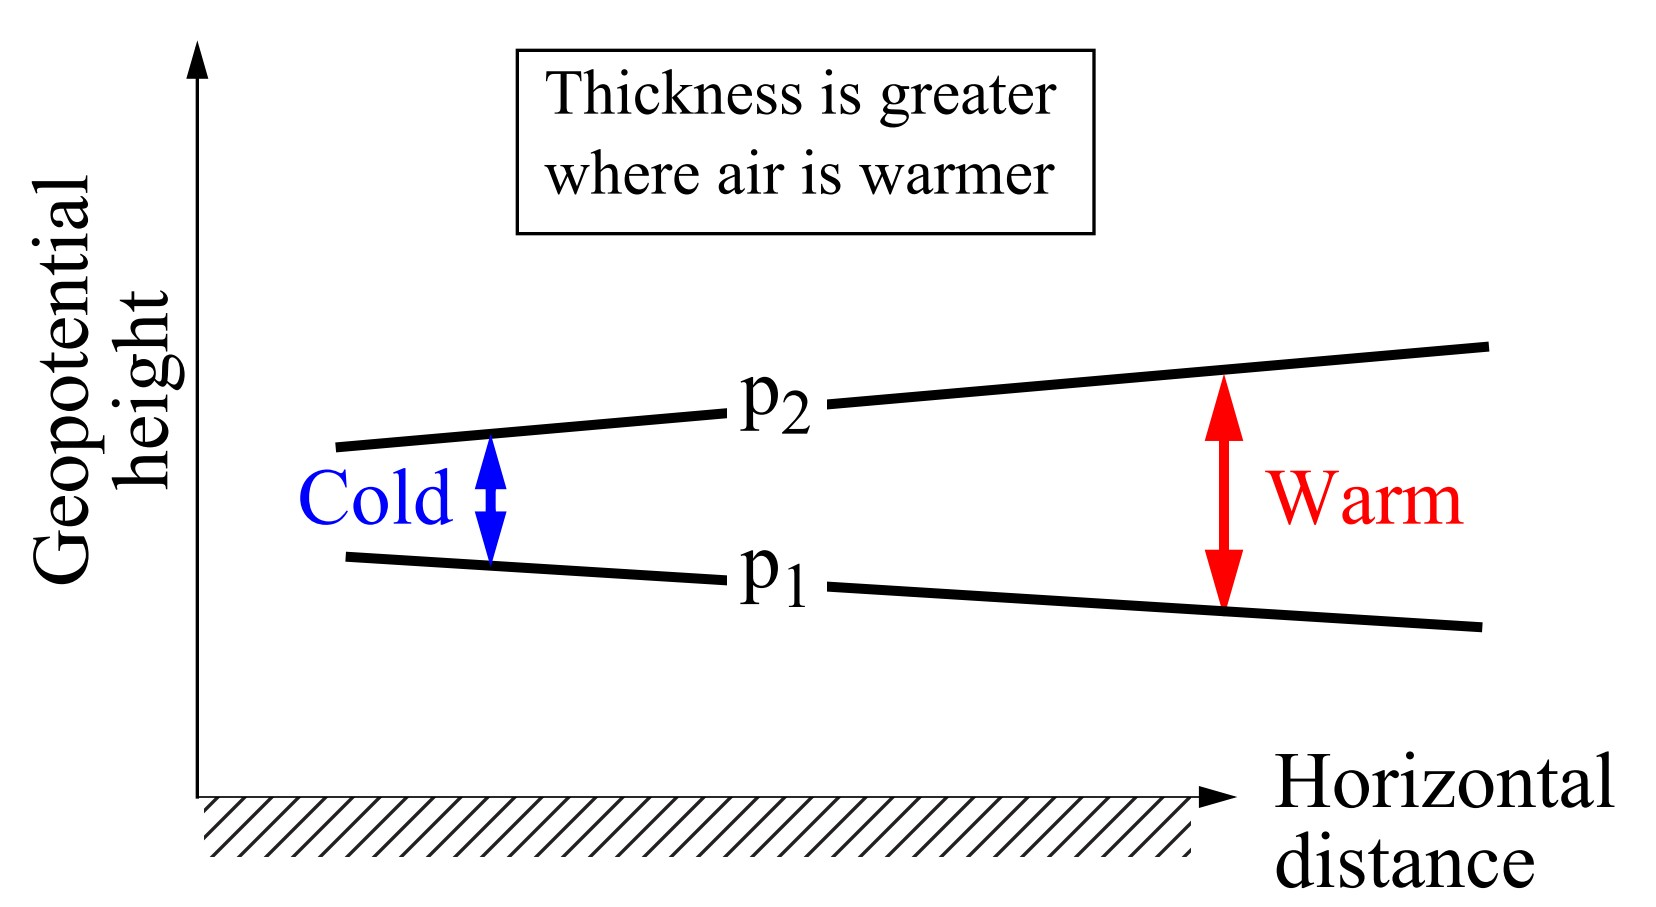
\includegraphics[width=7cm]{../figures/M2/pressure_thickness}
\end{columns}

\end{frame}
%
\begin{frame}{Pressure as a vertical coordinate}

\begin{columns}[t]

\column{7cm}
\begin{itemize}
\item {\footnotesize{}The primitive equations of atmospheric motion work
are easier to manage when pressure is substituted to geometric height.
When applied to the hydrostatic balance, it gives us an important
tool for characterising air masses }{\footnotesize\par}
\item {\footnotesize{}We can derive the formulation from the inversion of
the equation combining the hydrostatic equilibrium and the equation
of state (slide \pageref{frame:vertical-structure-pressure})}{\footnotesize\par}
\end{itemize}

\column{6cm}

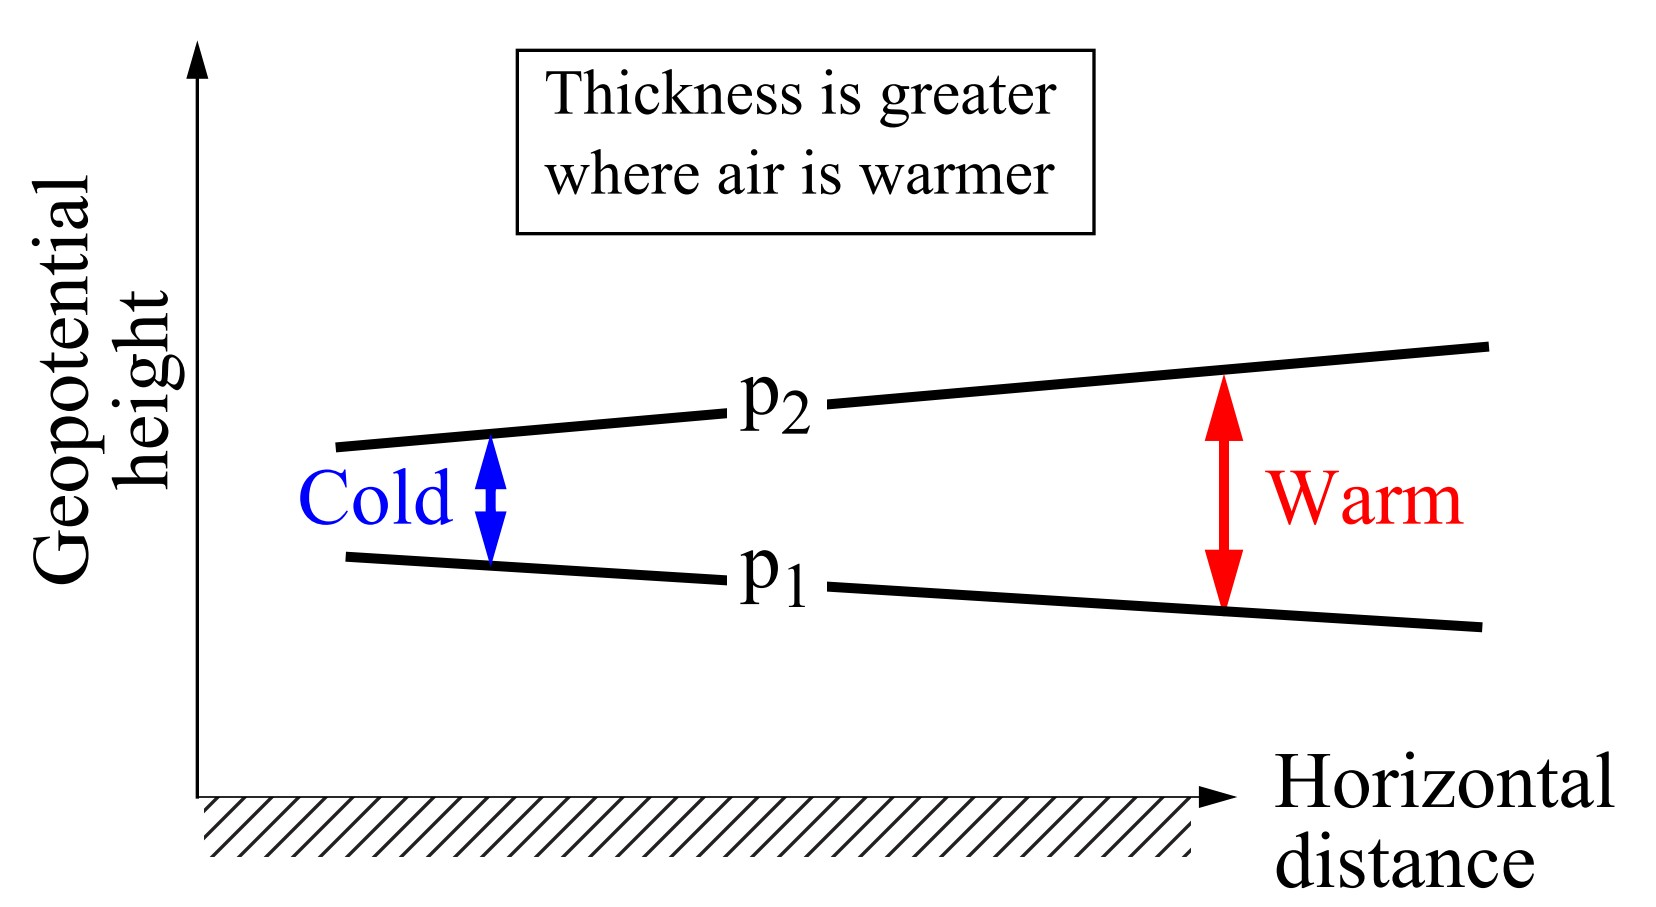
\includegraphics[width=6cm]{../figures/M2/pressure_thickness}
\begin{itemize}
\item {\footnotesize{}
\[
\frac{\partial p}{\partial z}=-\frac{gp}{RT}\rightarrow\frac{\partial z}{\partial p}=-\frac{RT}{gp}
\]
}{\footnotesize\par}
\item {\footnotesize{}This formulation can be integrated between two pressure
levels to yield the }\textbf{\footnotesize{}thickness of the layer}{\footnotesize{} }{\footnotesize\par}
\end{itemize}
\end{columns}

\end{frame}
%
\begin{frame}{Height of a pressure surface}

We integrate this equation from the reference surface pressure $p_{s}$
at mean sea level to obtain the \textbf{height} of a \textbf{surface
at a given pressure $p$} 
\[
\int_{p_{s}}^{p}\frac{\partial z}{\partial p'}dp'=\int_{p_{s}}^{p}-\frac{RT}{gp'}dp'
\]
\[
z(p)=R\int_{p}^{p_{s}}\frac{1}{g}\frac{T}{p'}dp'
\]
Note that we have swapped the integral extremes to change the sign
and $g$ stays in the integral. This height takes into account the
variation of gravity with latitude and height, and it is thus called
\textbf{geopotential height} (it incorporates the potential energy
of the air mass at that height). 
\end{frame}

\begin{frame}{Geopotential height (of pressure levels)}

\begin{definition}
The \textbf{geopotential height} is the height of an air mass in hydrostatic
equilibrium at a given pressure level $p$ , with respect to the surface
(the value of the gravity acceleration at the surface is used)
\[
z_{0}(p)=\frac{R}{g_{0}}\int_{p}^{p_{s}}\frac{T}{p'}dp'
\]
{\footnotesize{}Low height of a pressure surface in z-coordinates
corresponds to low pressure on a z surface (draw a straight line at
a given z, which is what we do for the MSLP). It also informs on the
temperature of the air masses up to that pressure level.}{\footnotesize\par}
\end{definition}

\begin{center}
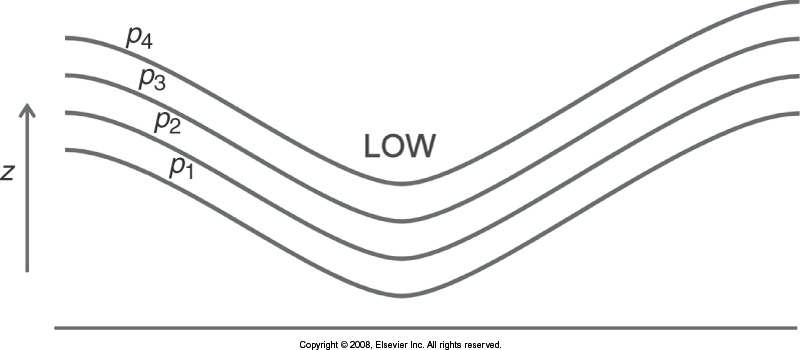
\includegraphics[width=7cm]{../figures/M2/f05-11-P558691}
\par\end{center}

\end{frame}

\begin{frame}{500 mb GH in the Northern Hemisphere}

\begin{columns}[t]


\column{7cm}
\begin{itemize}
\item The geopotential height is proportional to temperature, so where temperatures
are cold, air columns contract and geopotential heights are low, close
to ground.
\item The mean height of the \textbf{500 mb} pressure surface in January,
2003 (monthly mean, M\&P F5.12). The contour interval is \textbf{6
decameters = 60 m}. 
\item The surface is 5.88 km high in the tropics and 4.98 km high over the
pole
\end{itemize}

\column{6cm}
\begin{center}
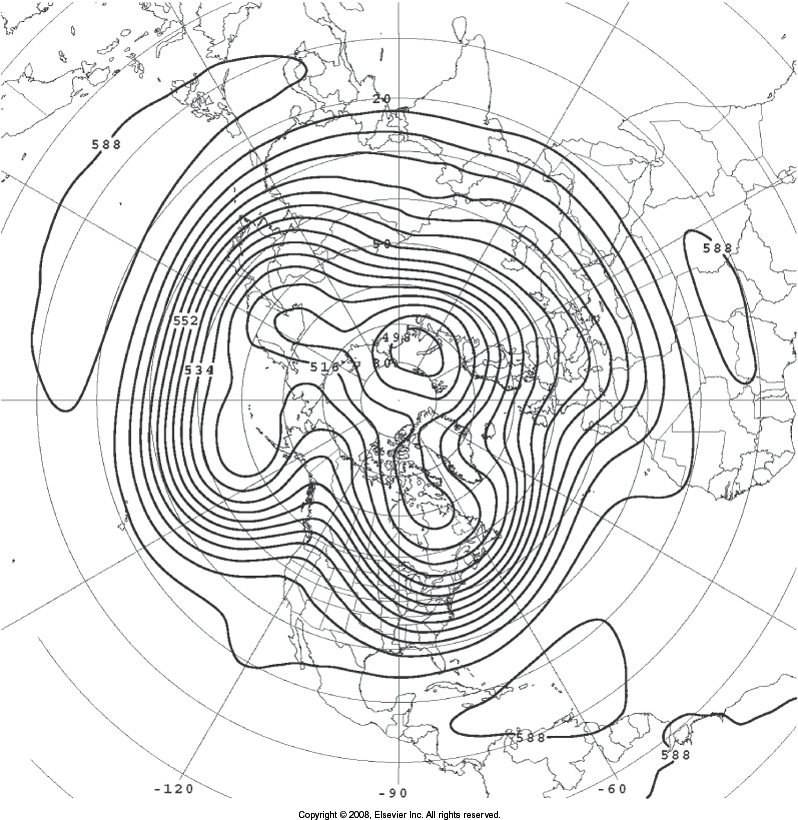
\includegraphics[width=6cm]{../figures/M2/f05-12-P558691}
\par\end{center}

\end{columns}

\end{frame}

\begin{frame}{500 mb GH in the Southern Hemisphere}

\begin{columns}[t]


\column{6cm}
\begin{itemize}
\item {\small{}S}{\footnotesize{}outhern Hemisphere }\textbf{\footnotesize{}mean
and anomaly}{\footnotesize{} of the}\textbf{\footnotesize{} 500 hPa}{\footnotesize{}
}\textbf{\footnotesize{}geopotential height}{\footnotesize{} for January
2015 (NCEP Reanalysis). Mean heights are denoted by solid contours
drawn at an interval of 8 dam }{\footnotesize\par}
\item {\footnotesize{}The anomaly contour interval is 3 dam with values
less (greater) than -3 dam (3 dam) indicated by blue (red) shading.
Anomalies are calculated as departures from the 1981-2010 climatology.}{\footnotesize\par}
\item {\footnotesize{}For the current conditions check out \url{https://www.cpc.ncep.noaa.gov/products/CDB/Extratropics/fige14.shtml}}{\footnotesize\par}
\end{itemize}

\column{5cm}

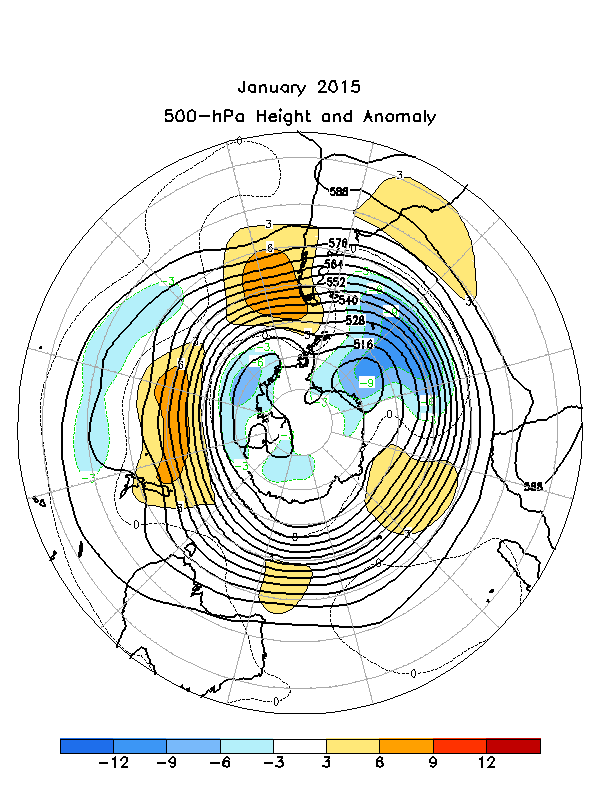
\includegraphics[width=5cm]{../figures/M2/GPheight_jan15}
\end{columns}

\end{frame}

\begin{frame}{Interannual variability}
\begin{center}
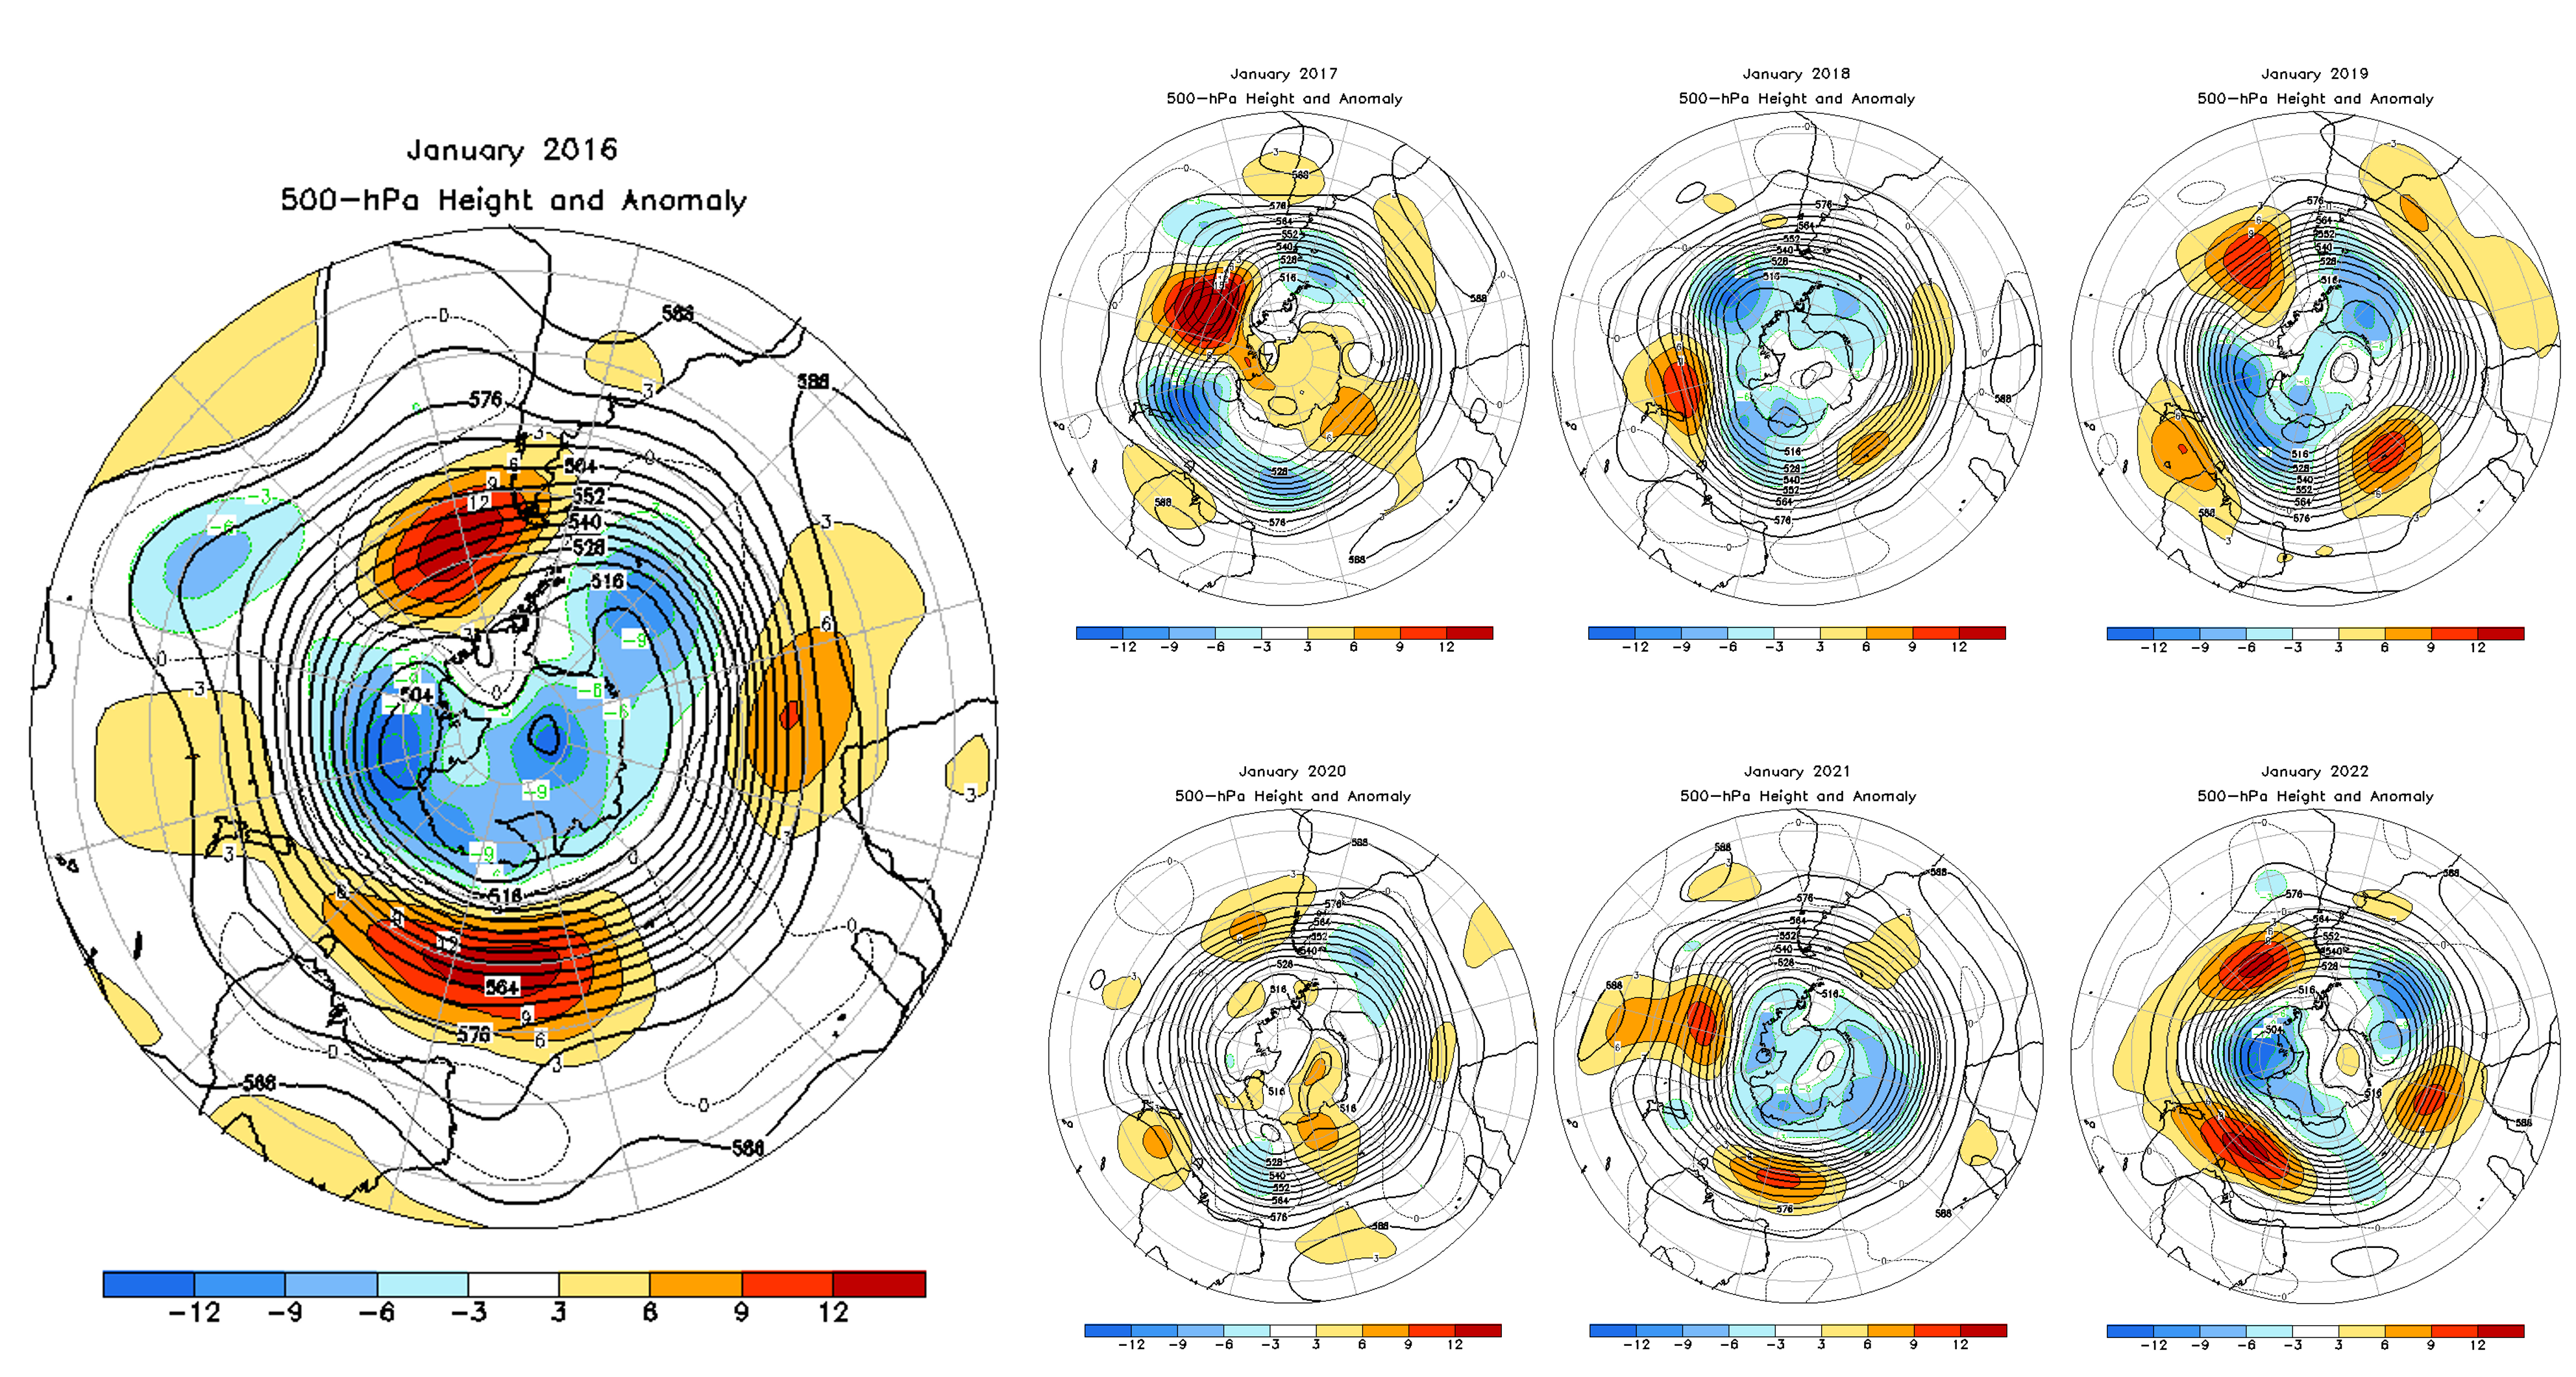
\includegraphics[width=12cm]{../figures/M2/GH_January_SH}
\par\end{center}

\end{frame}


\section{Stability and convection}
\begin{frame}{The nature of convection (M\&P, Chapter 4)}

\begin{columns}[t]


\column{8.3cm}
\begin{itemize}
\item {\footnotesize{}It is driven by }\textbf{\footnotesize{}buoyancy processes}{\footnotesize{}.
Buoyancy is the result of forces acting on an object (or portion of
the fluid) by a surrounding fluid.}{\footnotesize\par}
\item {\footnotesize{}When the }\textbf{\footnotesize{}ocean}{\footnotesize{}
is cooled from the atmosphere or warmed from below, it develops }\textbf{\footnotesize{}overturning
motion}{\footnotesize{}. This develops because the buoyancy of the
}\textbf{\footnotesize{}water parcel}{\footnotesize{} is modified
and the parcel density is not in equilibrium with the surrounding
waters. }\textbf{\footnotesize{}Density instabilities}{\footnotesize{}
modify the vertical structure of the ocean}{\footnotesize\par}
\item {\footnotesize{}At the Earth surface, the }\textbf{\footnotesize{}troposphere}{\footnotesize{}
is warmed by both direct solar radiation and downwelling terrestrial
radiation from the atmosphere. In radiative equilibrium, the surface
is warmer than the overlying atmosphere, creating an unstable condition
that leads to convective motion and to the resulting observed equilibrium
temperature}{\footnotesize\par}
\end{itemize}

\column{6.5cm}

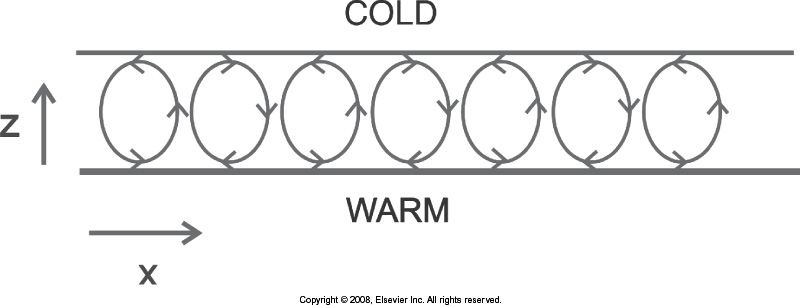
\includegraphics[width=6.6cm]{../figures/M2/f04-02-P558691}

~

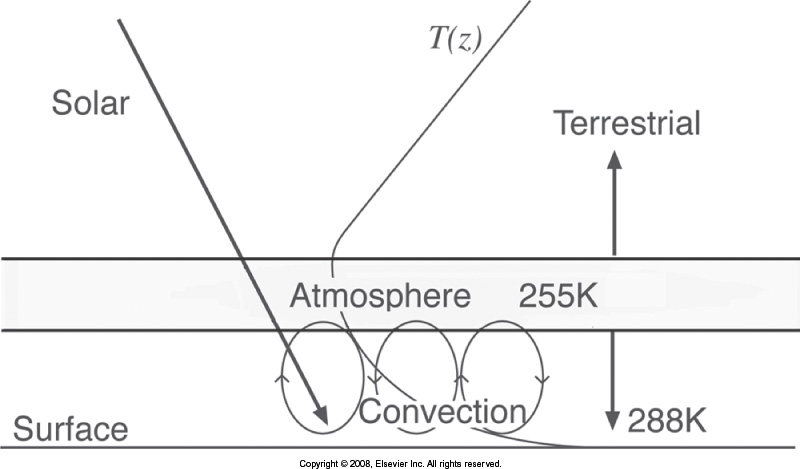
\includegraphics[width=6.6cm]{../figures/M2/f04-01-P558691}
\end{columns}

\end{frame}

\begin{frame}{Convection in the lab (M\&P, movie on Vula)}


\framesubtitle{\url{http://paoc.mit.edu/labweb/lab2/gfd_ii.htm}}
\begin{columns}[t]


\column{6cm}

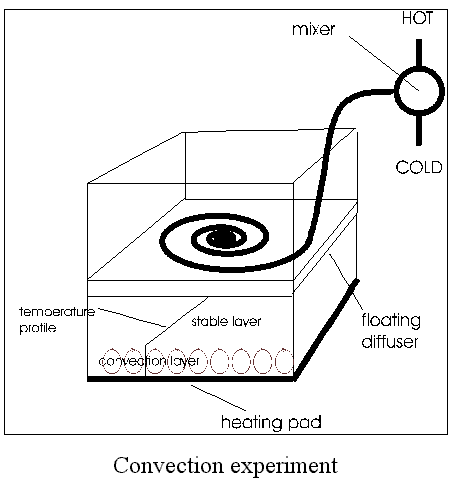
\includegraphics[scale=0.4]{../figures/M2/gfd_ii_convection}

\column{7cm}
\begin{itemize}
\item {\scriptsize{}A stable stratification can be set up in a 50 cm square
tank by slowly filling it up with water whose temperature is slowly
increased with time. This is done using (i) a mixer that mixes hot
and cold water together and (ii) a diffuser, which floats on the top
of the rising water and ensures that the warming water floats on the
top without generating turbulence.}{\scriptsize\par}
\item {\scriptsize{}The motion of the fluid is made visible by sprinkling
a VERY SMALL amount of potassium permanganate evenly over the base
of the tank. After switching on the heating at the base, thermals
will be seen to rise from the base, overshoot the level at which they
have zero buoyancy (the level where the T of the thermals is equal
to that of the environment) and sink back. Successive thermals rise
higher as the layer thickens.}{\scriptsize\par}
\end{itemize}
\end{columns}

\end{frame}
%
\begin{frame}{Convection in water: buoyancy}

\begin{columns}[t]


\column{7cm}
\begin{itemize}
\item {\footnotesize{}Water can be considered an }\textbf{\footnotesize{}incompressible
fluid}{\footnotesize{} and therefore its density is mostly affected
by temperature and salinity changes. If a parcel of water is warmer,
then it will be less dense than the surrounding. The hydrostatic balance
will generate a pressure difference and the parcel will rise. }\textbf{\footnotesize{}What
is the acceleration of this motion?}{\footnotesize{} }{\footnotesize\par}
\item {\footnotesize{}It is not just $g,$but it depends on the relative
difference of density between the parcel and the surrounding. We call
this acceleration (or force), the }\textbf{\footnotesize{}buoyancy
}{\footnotesize{}($z$ axis oriented upward): 
\[
b=-g\frac{\rho_{P}-\rho_{E}}{\rho_{E}}
\]
}{\footnotesize\par}
\end{itemize}

\column{6.5cm}

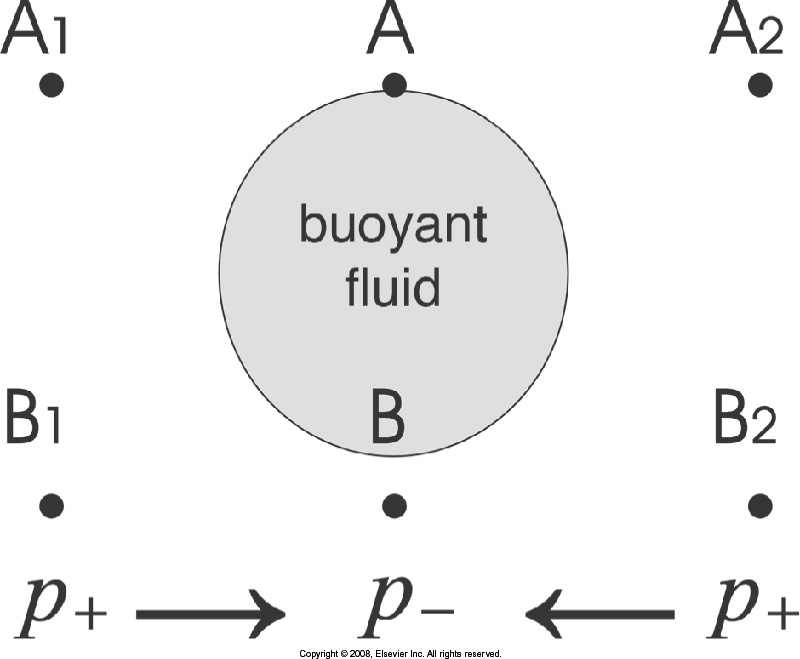
\includegraphics[width=6cm]{../figures/M2/f04-04-P558691}
\begin{itemize}
\item {\footnotesize{}Depending on the density of the parcel with respect
to the surrounding, we have }\textbf{\footnotesize{}positive}{\footnotesize{}
(rise), }\textbf{\footnotesize{}negative}{\footnotesize{} (sink) or
}\textbf{\footnotesize{}neutral}{\footnotesize{} (stationary) }\textbf{\footnotesize{}buoyancy}{\footnotesize\par}
\end{itemize}
\end{columns}

\end{frame}

\begin{frame}{Convection in a compressible atmosphere}
\label{frame:compress_atm}

\begin{columns}[t]


\column{9cm}
\begin{itemize}
\item {\footnotesize{}The atmosphere is a }\textbf{\footnotesize{}compressible
fluid}{\footnotesize{} and density is governed by the equation of
state $\rho=p/RT$}{\footnotesize\par}
\item {\footnotesize{}When an air mass is warmed by the sun or from the
ocean below, it gains heat (}\textbf{\footnotesize{}diabatic process}{\footnotesize{}).
When it is displaced by convection }\textbf{\footnotesize{}the parcel
changes its volume}{\footnotesize{} from one pressure level to another
(think of the perfect gas law $pV=nR_{g}T$ if $T$ is kept constant).
This is an }\textbf{\footnotesize{}adiabatic process}{\footnotesize{}
that does not involve any heat exchange.}{\footnotesize\par}
\item {\footnotesize{}The parcel at $z=z_{1}$ with $\rho_{1}=p(z_{1})/RT(z_{1})$
is stable with respect to $\rho_{2}=p(z_{2})/RT(z_{2})$. If the air
parcel is }\textbf{\footnotesize{}adiabatically}{\footnotesize{} displaced
to level $z_{2}$ by convection, the environmental pressure decreases,
the volume expands and some }\textbf{\footnotesize{}work}{\footnotesize{}
is done on the surrounding: $dW=pdV$ }{\footnotesize\par}
\item {\footnotesize{}The 1st law of thermodynamics $\delta Q=dU+pdV$ tells
us that if there is some volume change and no exchange of }\textbf{\footnotesize{}heat}{\footnotesize{}
$Q$, then the }\textbf{\footnotesize{}internal energy}{\footnotesize{}
$U$ must be reduced, with a consequent cooling of the parcel.}{\footnotesize\par}
\end{itemize}

\column{5cm}

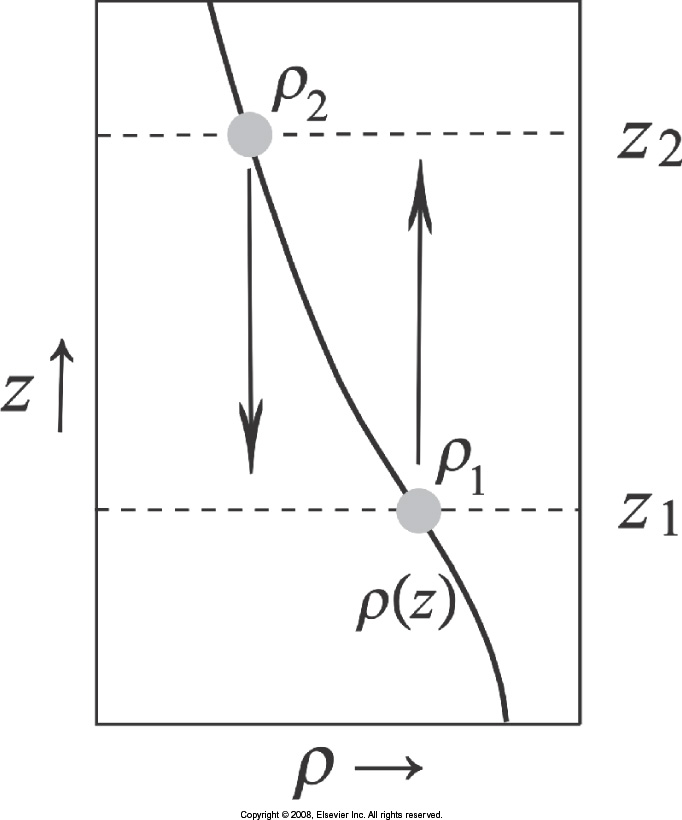
\includegraphics[width=4cm]{../figures/M2/f04-05-P558691}

\textbf{\footnotesize{}What is the new temperature of the parcel and
how does it affect the buoyancy?}{\footnotesize\par}
\end{columns}

\end{frame}
%
\begin{frame}{Lapse rates}

{\small{}We have seen that temperature changes with altitude. This
change, the vertical gradient $\partial T/\partial z$, is called
the }\textbf{\small{}lapse rate}{\small{} (lapse=interval). A negative
lapse rate represents the normal condition with cooler air above.
The opposite, a positive lapse rate (ie the temperature increases
with height) is called an inversion. Mean profiles from various regions
and from hourly radiosonde data close to Sidney are shown below (Climate
and Weather Explained, Linacre and Geerts, 1997). The }\textbf{\small{}Environmental
Lapse Rate}{\small{} (ELR) at each level is the }\textbf{\small{}tangent
to the profile}{\small{}.}{\small\par}

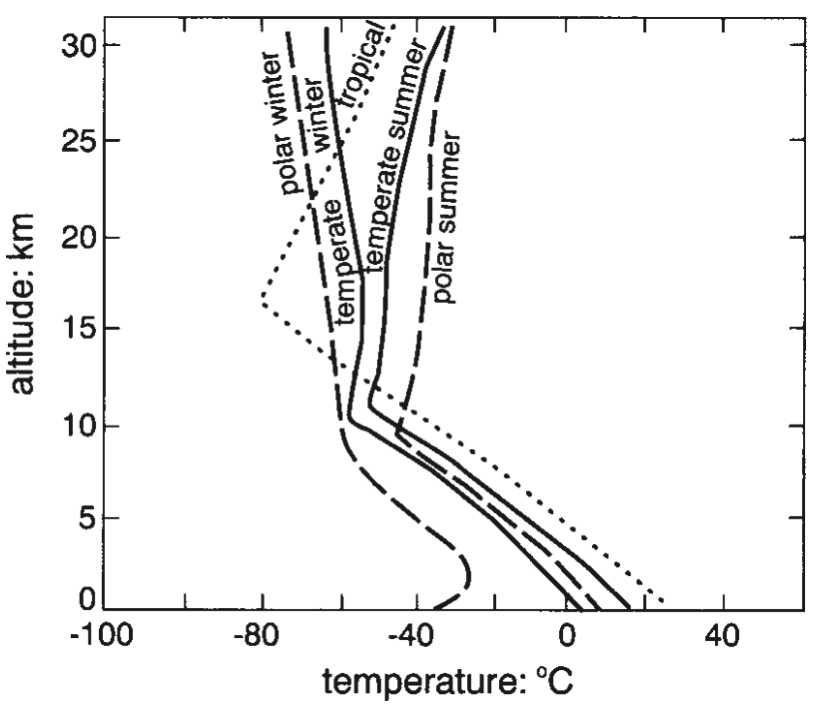
\includegraphics[width=5cm]{../figures/M2/lapse_rates}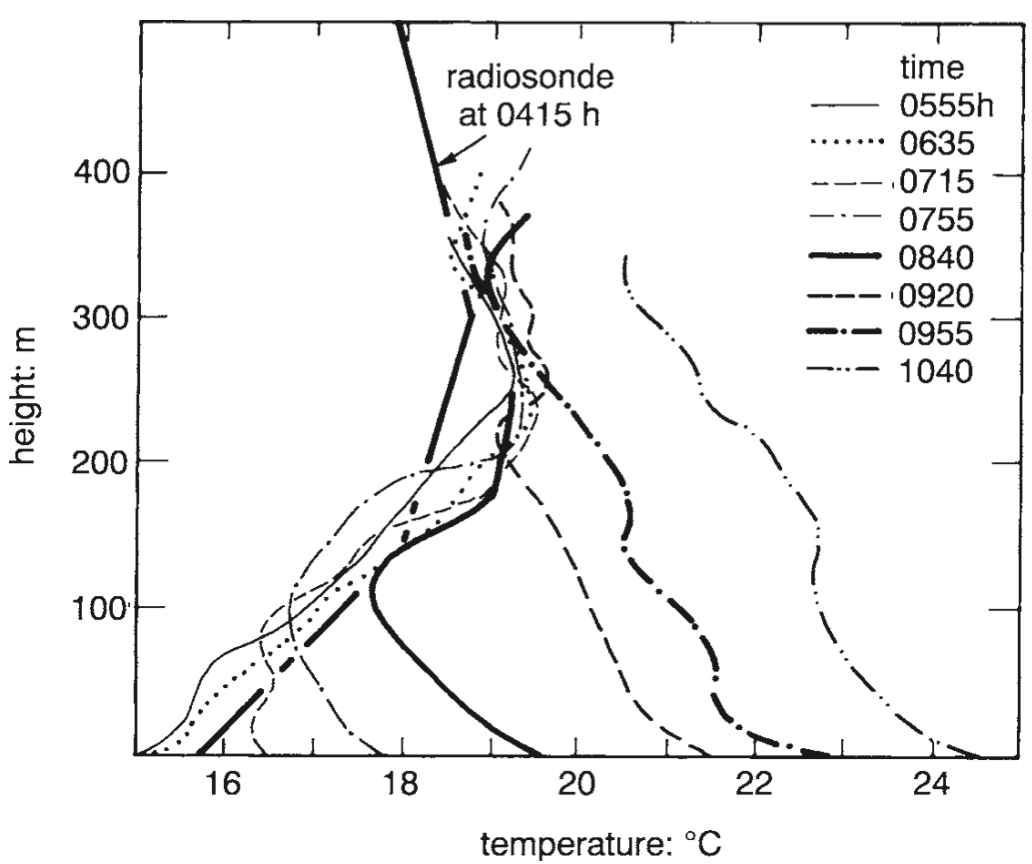
\includegraphics[width=5cm]{../figures/M2/lapse_rates_sideny}
\end{frame}

\begin{frame}{The dry adiabatic lapse rate (DALR)}

\begin{itemize}
\item {\small{}We can derive a theoretical lapse rate for an ascending or
descending parcel of dry air. It quantifies how the $T$ of a parcel
of air changes during }\textbf{\small{}adiabatic motion}{\small{}
using the 1st law of thermodynamics
\[
\delta Q=dU+pdV=0
\]
 }{\small\par}
\item {\small{}The first law can be rewritten with (quite) some algebra
in terms of specific heats ($c_{p},\,c_{v}$) and using the equation
of state we get
\[
\delta Q=c_{v}dT+pdV=\left(R+c_{v}\right)dT-\frac{dp}{\rho}=c_{p}dT-\frac{dp}{\rho}=0
\]
}{\small\par}
\item {\small{}Using the hydrostatic balance, we can include a description
of the pressure differential $\left(dp=-g\rho dz\right)$ that yields
\[
\boxed{\mathsf{DALR=}\frac{dT}{dz}=-\frac{g}{c_{p}}=-\Gamma_{d}}
\]
with $c_{p}=1005$ J kg$^{-1}$ K$^{-1}$ and the constant $\Gamma_{d}\simeq10$
K km$^{-1}$. }\textbf{\small{}Note that we call DALR the temperature
gradient, not the constant }{\small{}$\Gamma_{d}$.}{\small\par}
\end{itemize}
\end{frame}

\begin{frame}{Stability and instability: a conceptual explanation}

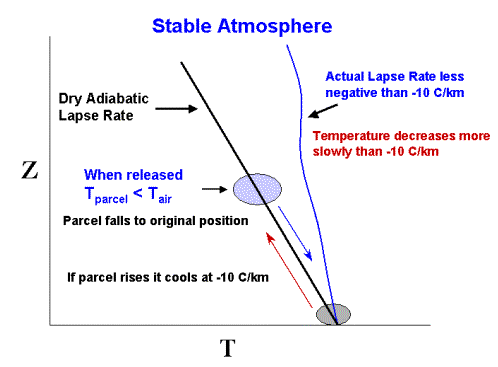
\includegraphics[width=6.5cm]{../figures/M2/stable_dry}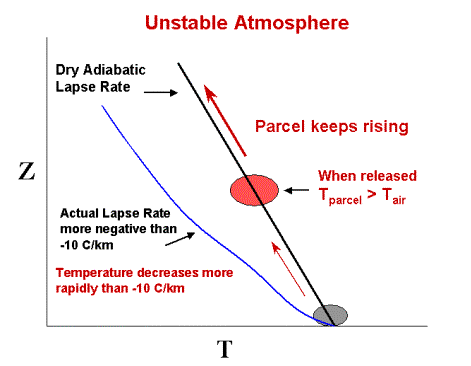
\includegraphics[width=6.5cm]{../figures/M2/unstable_dry}

Depends on the relationship between the (theoretical) dry adiabatic
lapse rate and the environmental lapse rate:

$ELR>DALR\Rightarrow$STABLE; $ELR<DALR\Rightarrow$UNSTABLE; $ELR\simeq DALR\Rightarrow$NEUTRAL
\end{frame}

\begin{frame}{The density of an uplifted dry parcel}

\begin{columns}[t]


\column{11cm}
\begin{itemize}
\item {\footnotesize{}To determine whether there will be a buoyancy force
acting on the displaced parcel we must compare its density to the
one of the surrounding environment}{\footnotesize\par}
\item {\footnotesize{}Considering again the figure at pag. \pageref{frame:compress_atm},
we have
\begin{align*}
\rho_{2} & =\rho(z_{2})=p_{2}/RT_{2}\\
T(z_{2}) & =T_{1}+\left(dT/dz\right)_{E}\Delta z
\end{align*}
where $\Delta z=\left(z_{2}-z_{1}\right)$. The temperature of the
parcel follows the adiabatic lapse rate 
\[
T_{P}=T_{1}-\Gamma_{d}\Delta z
\]
 and we compute the density from the equation of state
\[
\rho_{P}=p_{2}/\left(RT_{P}\right)
\]
To determine the buoyancy pull, we check if the density of the parcel
$\rho_{P}$ is larger, lower of equal to the surrounding $\rho_{2}$ }{\footnotesize\par}
\end{itemize}

\column{5cm}

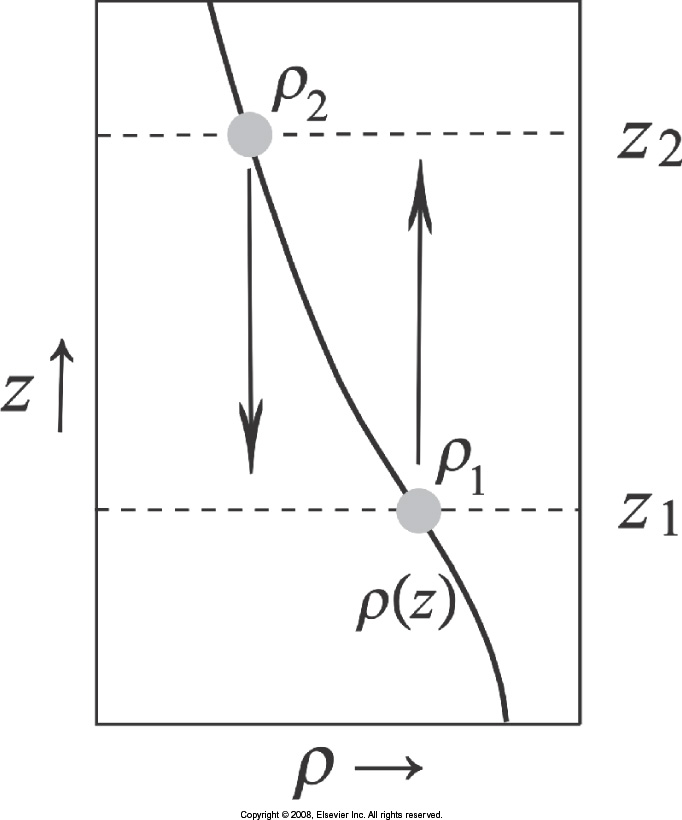
\includegraphics[width=4cm]{../figures/M2/f04-05-P558691}
\end{columns}

\end{frame}
%
\begin{frame}{Stability conditions}

\begin{itemize}
\item {\footnotesize{}Since density is only determined by temperature, all
this is simplified by comparing the lapse rates 
\[
T_{P}=T_{1}-\Gamma_{d}\Delta z\left(\lesseqqgtr\right)T_{1}+\left(\frac{dT}{dz}\right)_{E}\Delta z=T_{2}
\]
}{\footnotesize\par}
\begin{itemize}
\item {\footnotesize{}$\left(\frac{dT}{dz}\right)_{E}>-\Gamma_{d}$ the
displaced parcel is }\textbf{\footnotesize{}colder}{\footnotesize{}
and the atmosphere is }\textbf{\footnotesize{}stable}{\footnotesize\par}
\item {\footnotesize{}$\left(\frac{dT}{dz}\right)_{E}<-\Gamma_{d}$ the
displaced parcel is }\textbf{\footnotesize{}warmer}{\footnotesize{}
and the atmosphere is }\textbf{\footnotesize{}unstable}{\footnotesize\par}
\item {\footnotesize{}$\left(\frac{dT}{dz}\right)_{E}=-\Gamma_{d}$ the
atmosphere is }\textbf{\footnotesize{}neutral}{\footnotesize\par}
\end{itemize}
\item {\footnotesize{}In the tropics, the lower troposphere $\left(dT/dz\right)_{E}\simeq-4.5$
K km$^{-1}$, less negative than -$\Gamma_{d}$. The atmosphere is
in general stable to dry convection. It is the release of }\textbf{\footnotesize{}latent
heat due to condensation}{\footnotesize{} that makes it unstable}{\footnotesize\par}
\end{itemize}
\end{frame}

\begin{frame}{Local instability}

\begin{columns}[t]

\column{6cm}
\begin{center}
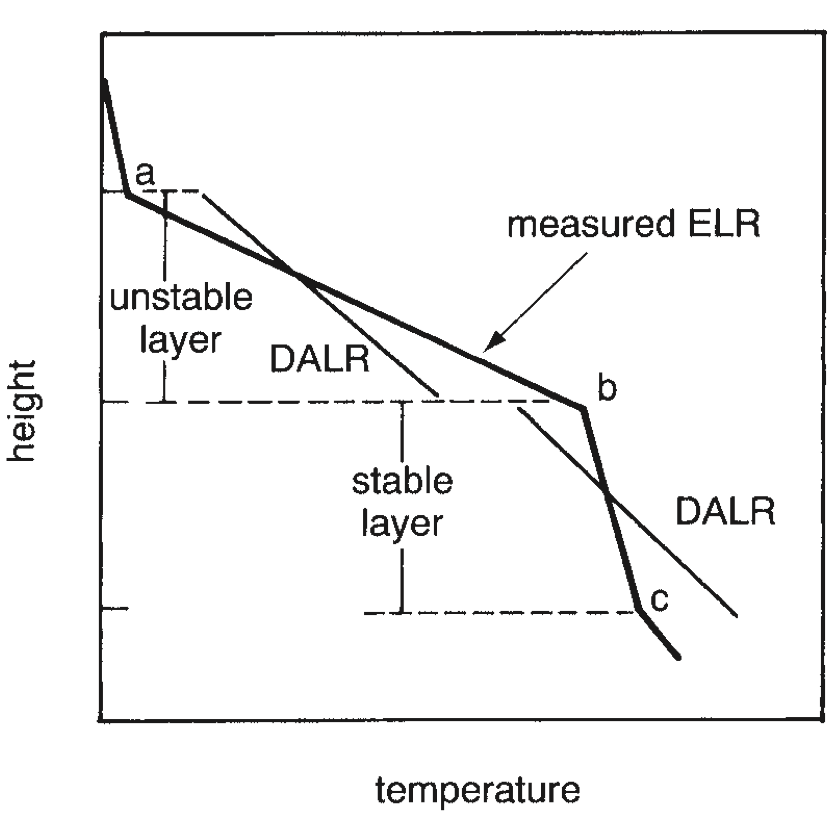
\includegraphics[width=6cm]{../figures/M2/local_instability}
\par\end{center}

\column{6cm}

A comparison of the dry adiabatic lapse rate (DALR) with the environmental
lapse rate (ELR) in each of two layers. The top one is unstable and
the bottom one is stable

The atmospheric local static stability corresponds to an ELR more
clockwise than the DALR. ({\small{}Climate and Weather Explained,
Linacre and Geerts, 1997)}{\small\par}
\end{columns}

\end{frame}

\begin{frame}{Moist air: Condensation}

\begin{itemize}
\item {\footnotesize{}The main forms of condensation are clouds, mostly
at high levels, and fogs, at or near the ground. These forms of condensation
occur when air is brought to saturation point or temperature decreased
to the dew-point. Condensation is assisted in the atmosphere by condensation
nuclei around which liquid water can form. Condensation does not always
lead to precipitation; gravity has to overcome the winds that keep
the water vapour buoyant before this can occur. Most saturation and
condensation processes in the atmosphere take place as a result of
air cooling, principally by the vertical ascent of air \url{http://www.memonic.com/user/pyuhun/folder/all/id/1iTHA}}{\footnotesize\par}
\item {\footnotesize{}Air is forced to rise and cool by:}

\begin{itemize}
\item {\footnotesize{}orographic uplift}{\footnotesize\par}
\item {\footnotesize{}frontal uplift}{\footnotesize\par}
\item {\footnotesize{}large-scale convergence and ascent in low-pressure
tropical systems}{\footnotesize\par}
\item {\footnotesize{}smaller-scale convective currents}{\footnotesize\par}
\end{itemize}
\end{itemize}
\end{frame}

\begin{frame}{Types of convection}

\begin{columns}[t]

\column{7cm}
\begin{center}
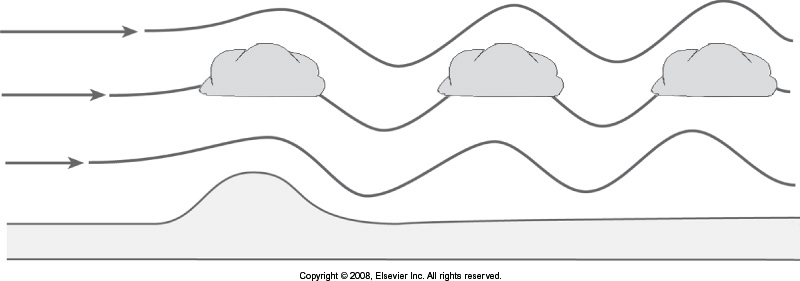
\includegraphics[width=7cm]{../figures/M2/f04-13-P558691}
\par\end{center}

Orographic uplift and cloud formation due to gravity waves in the
wake of a mountain

\column{6cm}

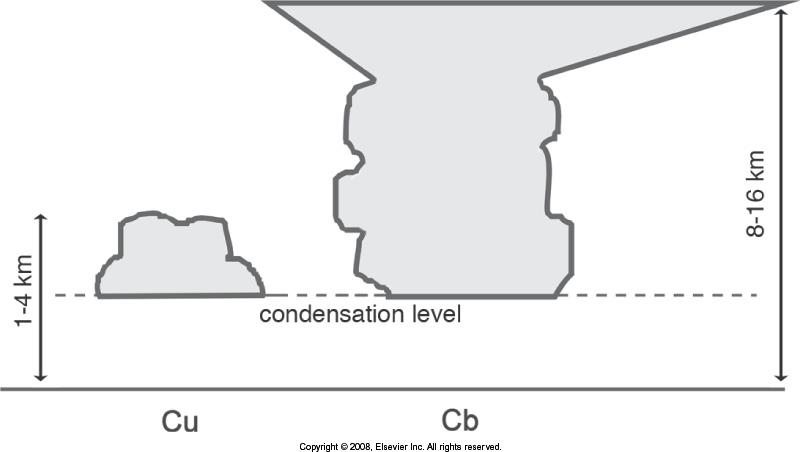
\includegraphics[width=7cm]{../figures/M2/f04-20-P558691}

{\small{}Convective clouds have two main forms: Cumulus (Cu, capped,
fair weather and non-precipitating) and Cumulonimbus (Cb, heavy rain
and storms) }{\small\par}
\end{columns}

\end{frame}
%
\begin{frame}{Convective clouds}
\begin{columns}[c]

\column{7cm}
\begin{itemize}
\item {\small{}Once the air reaches the condensation level, it saturates
and there is an }\textbf{\small{}exchange of heat}{\small{}. }{\small\par}
\item {\small{}Water vapour is formed, latent heat is released during water
condensation and the air warms and raises further creating the typical
tropical clouds (cumulonimbus). For a cool intro to clouds, see \url{https://www.ted.com/talks/gavin_pretor_pinney_cloudy_with_a_chance_of_joy } }{\small\par}
\item {\small{}The process is not adiabatic and the DALR does not hold any
more}{\small\par}
\end{itemize}

\column{6cm}

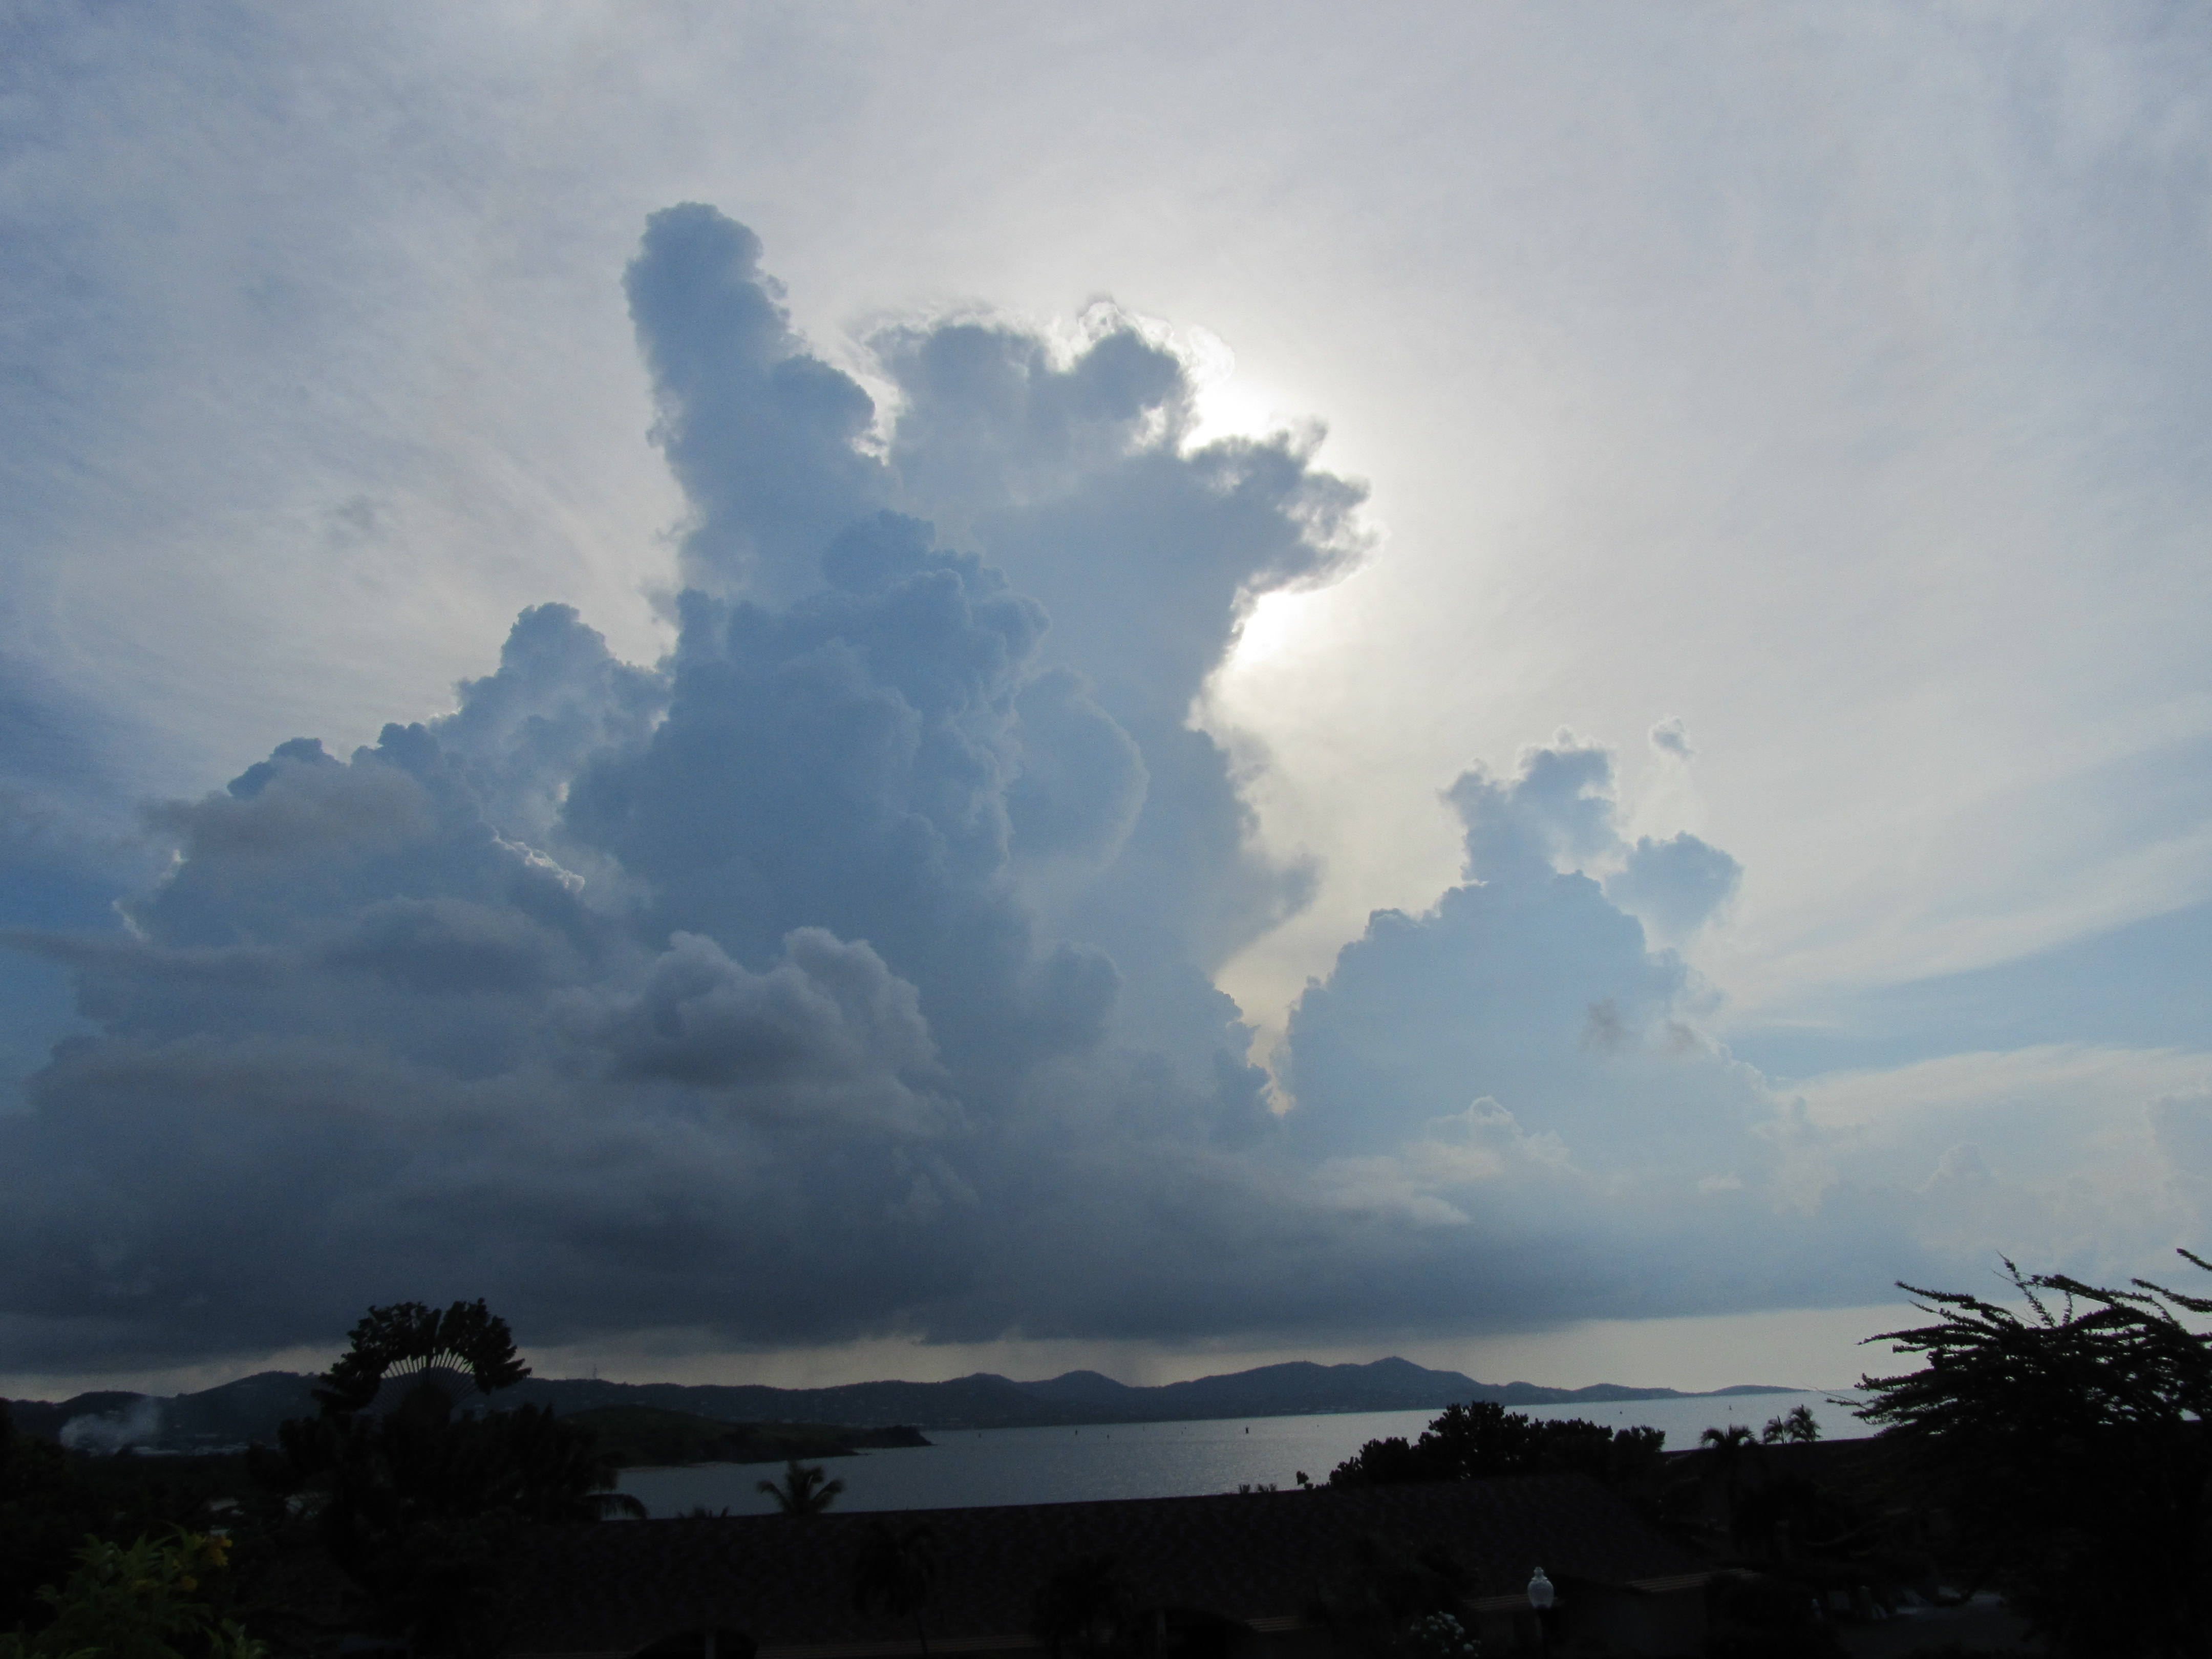
\includegraphics[width=6.5cm]{../figures/M2/tropicalcloud.JPG}
\end{columns}

\end{frame}

\begin{frame}{The saturated (wet) adiabatic lapse rate (SALR)}

\begin{columns}[t]


\column{7.5cm}

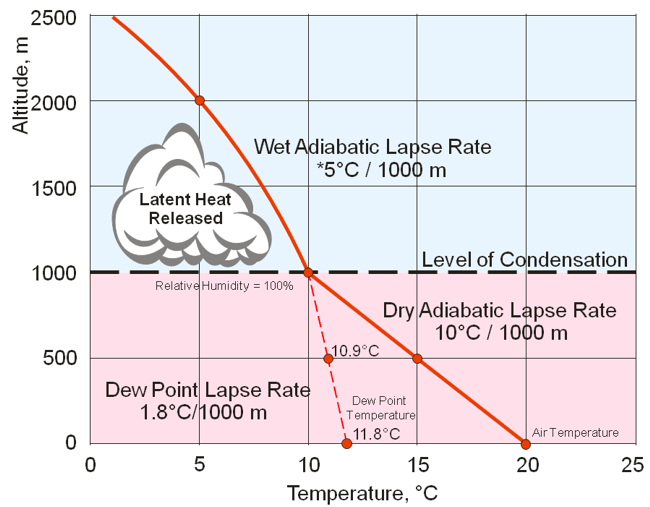
\includegraphics[width=8cm]{../figures/M2/SALR}
\begin{itemize}
\item {\footnotesize{}The ELR of the tropical troposphere is similar to
the SALR (neutral). A state called }\textbf{\footnotesize{}conditional
instability}{\footnotesize{} }{\footnotesize\par}
\end{itemize}

\column{7cm}
\begin{itemize}
\item {\footnotesize{}The adiabatic lapse rate is modified by the release
of heat due to condensation 
\[
\Gamma_{s}=\Gamma_{d}\left[\frac{1+Lq_{s}/RT}{1+\beta Lq_{s}/c_{p}}\right]
\]
where we used the simplified Clausius-Clapeyron equation, $L$ is
latent heat and $q_{s}$ is the saturation-specific humidity (also
$q_{*}$). The value in brackets is always smaller than 1 and SALR
varies between 3 K km$^{-1}$ in the lower tropical atmosphere to
10 in the upper drier troposphere}{\footnotesize\par}
\item {\footnotesize{}the }\textbf{\footnotesize{}release of latent heat}{\footnotesize{}
makes the rising parcel warmer and the atmosphere is destabilized
by the presence of water vapour }{\footnotesize\par}
\end{itemize}
\end{columns}

\end{frame}

\begin{frame}{Stability and Conditional instability}

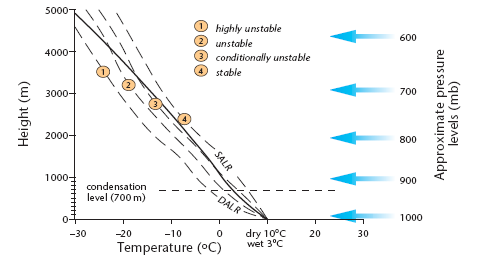
\includegraphics[scale=0.6]{../figures/M2/conditional}

{\footnotesize{}The relationship between the ELR and both the DALR
and the SALR describes how temperature changes with height, and thus
the density and buoyancy of a vertically displaced parcel in comparison
with its atmospheric surroundings. It thus determines air stability
and what happens to the displaced air parcel }{\footnotesize\par}
\end{frame}


\end{document}
